\documentclass[a4paper, twoside]{article}
\title{\vspace{20cm}\fontsize{50pt}{40pt}\selectfont{All-in at the River}\\\fontsize{24pt}{\baselineskip}\selectfont{Standard Code Library}\vspace{0.1cm}}
\author{\fontsize{15pt}{\baselineskip}\selectfont{Shanghai Jiao Tong University}\vspace{0.2cm}\\\fontsize{11pt}{\baselineskip}\selectfont{Desprado2\quad fstqwq\quad AntiLeaf}}
\date{}

% green= '#10BC72' # '#C3E88D'
% cyan= '#00A1D6' # '#89DDFF'

% \usepackage{zxjatype}
% \setjamainfont{ipaexm.ttf}

\usepackage{graphicx, amssymb, amsmath, textcomp, booktabs}
% \usepackage[libertine, vvarbb]{newtxmath}
\usepackage[scr=rsfso]{mathalfa}
%\usepackage[lining, semibold, type1]{libertine} % a bit lighter than Times--no osf in math
\usepackage[T1]{fontenc} % best for Western European languages
\usepackage{minted}
\usepackage{listings, color, setspace, titlesec, fancyhdr, mdframed, multicol}
\usepackage{fontspec}
\usepackage{ucharclasses}
\usepackage{xunicode, xltxtra}
\usepackage{pdfpages}
\usepackage{tocloft}
\usepackage{nameref}
\usepackage{verbatim}
\usepackage{relsize}
\usepackage[normalem]{ulem}
\usepackage[colorlinks, linkcolor = black]{hyperref}
\usepackage{color,xcolor}
\usepackage{afterpage}
\usepackage{xeCJK}
\usepackage{enumitem}

\setenumerate[1]{itemsep=5pt,partopsep=0pt,parsep=\parskip,topsep=5pt,itemindent=1em,leftmargin=3pt}
\setitemize[1]{itemsep=0pt,partopsep=0pt,parsep=\parskip,topsep=5pt,itemindent=1em,leftmargin=3pt}
\setdescription{itemsep=0pt,partopsep=0pt,parsep=\parskip,topsep=5pt,itemindent=1em,leftmargin=3pt}

\setlength{\itemindent}{0em}
\setlength\parindent{0em}

\definecolor{light-gray}{gray}{0.9}    % 1.灰度
\definecolor{black}{gray}{0.0}

%configure space between the two columns
\setlength{\columnsep}{13pt}

\setCJKmainfont{等线}[Scale=0.9]
\setCJKmonofont{SimHei}[Scale=0.9]
\setCJKsansfont{KaiTi}[Scale=0.9]
%\setmainfont{TeX Gyre Pagella} % [Scale=1]
\setmonofont{Cascadia Code} [Scale=0.8]
% \newfontfamily\substitutefont{等线}[Scale=0.9]
% \setTransitionsForChinese{\begingroup\substitutefont}{\endgroup}
\XeTeXlinebreaklocale "zh"
\XeTeXlinebreakskip = 0pt plus 1pt

%configure minted to display codes
\definecolor{Gray}{rgb}{0.9,0.9,0.9}

%configure section style of table of content
\renewcommand\cftsecfont{\Large}

%configure section style
\titleformat{\section}
{\huge\bfseries}			% The style of the section title
{\thesection }				% a prefix
{15pt}						% How much space exists between the prefix and the title
{}					% How the section is represented
% \titleformat{\section}{\huge}{}{0pt}{}
% \titlespacing{\section}{0pt}{0pt}{0pt}
% \titlespacing{\subsection}{0pt}{0pt}{0pt}
% \titlespacing{\subsubsection}{0pt}{0pt}{0pt}

\usepackage{fancyhdr}
\usepackage[inner=0.7cm, outer=1.0cm, top=1.7cm, bottom=0.4cm]{geometry}
% inner = 1.35cm, outer = 0.9cm

\usepackage{wallpaper}
\usepackage{color}

\setlength{\headsep}{0.1cm}
\setlength{\footskip}{0.7cm}

\fancypagestyle{fancy} {

	% \pagestyle{fancy}

	\chead{Standard Code Library}
	\lhead{\nouppercase\leftmark}
	\rhead{\nouppercase\rightmark}
	\cfoot{\thepage}

}

\renewcommand{\headrulewidth}{0.5pt}
\renewcommand{\footrulewidth}{0.5pt}

\mathchardef\mhyphen="2D

\setminted[cpp]{
	style=solarized-light,
	mathescape,
	linenos,
	autogobble,
	baselinestretch=0.9,
	tabsize=4,
	fontsize=\normalsize,
	%bgcolor=Gray,
	frame=single,
	framesep=1mm,
	framerule=0.3pt,
	numbersep=1mm,
	breaklines=true,
	breaksymbolsepleft=2pt,
	%breaksymbolleft=\raisebox{0.8ex}{ \small\reflectbox{\carriagereturn}}, %not moe!
	%breaksymbolright=\small\carriagereturn,
	breakbytoken=false,
	showtabs=true,
	tab={\relscale{1.08} $\color{light-gray}{\vert} \ \ \ $ \relscale{1}},
}

\setminted[python]{
	style=solarized-light,
	mathescape,
	linenos,
	autogobble,
	baselinestretch=0.9,
	tabsize=4,
	fontsize=\normalsize,
	%bgcolor=Gray,
	frame=single,
	framesep=0.8mm,
	framerule=0.3pt,
	numbersep=0.8mm,
	breaklines=true,
	breaksymbolsepleft=2pt,
	%breaksymbolleft=\raisebox{0.8ex}{ \small\reflectbox{\carriagereturn}}, %not moe!
	%breaksymbolright=\small\carriagereturn,
	breakbytoken=false,
	showtabs=true,
	tab={\relscale{1.08} $\color{light-gray}{\vert} \ \ \ $ \relscale{1}},
}

\begin{document}

	\begin{titlepage}
		\ThisCenterWallPaper{1.1}{image/73564338_p0.jpg}

% \textrm{TeX Gyre Pagella}

\fontspec{TeX Gyre Pagella}\selectfont{\color{white}{
	\maketitle
	
	\centerline{Last Commit: \input{|"python ../src/cover/last-commit.py"}}
}}

\thispagestyle{empty}

	\end{titlepage}

	\pagestyle{plain}

	\pagenumbering{roman}
	\setcounter{page}{1}

	\begin{multicols}{2}
		
		\begin{spacing}{1}
			% \renewcommand{\contentsname}{\huge{目录}}
			\tableofcontents
		\end{spacing}

	\end{multicols}

	\newpage

	\pagestyle{fancy}

	\pagenumbering{arabic}
	\setcounter{page}{1}

	\begin{multicols}{2}
		\section{数学}
			
			\subsection{多项式}
				\subsubsection{FFT}
					\inputminted{cpp}{../src/math/FFT.cpp}

				\subsubsection{NTT}
					\inputminted{cpp}{../src/math/NTT.cpp}

				\subsubsection{任意模数卷积 (MTT, 毛梯梯)}
					三模数NTT和直接拆系数FFT都太慢了, 不要用.

MTT的原理就是拆系数FFT, 只不过优化了做变换的次数.

考虑要对$A(x)$, $B(x)$两个多项式做DFT, 可以构造两个复多项式

$$ P(x) = A(x) + iB(x) \quad Q(x) = A(x) - iB(x) $$

只需要DFT一个, 另一个DFT实际上就是前者反转再取共轭, 再利用

$$ A(x) = \frac {P(x) + Q(x)} 2 \quad B(x) = \frac {P(x) - Q(x)} {2i} $$

即可还原出$A(x)$, $B(x)$.

IDFT的道理更简单, 如果要对$A(x)$和$B(x)$做IDFT, 只需要对$A(x) + i B(x)$做IDFT即可, 因为IDFT的结果必定为实数, 所以结果的实部和虚部就分别是$A(x)$和$B(x)$.

\textbf{实际上任何同时对两个实序列进行DFT, 或者同时对结果为实序列的DFT进行逆变换时都可以按照上面的方法优化, 可以减少一半的DFT次数.}

\inputminted{cpp}{../src/math/MTT.cpp}
			
				\subsubsection{多项式操作}
					\label{PolyOperation}
					\inputminted{cpp}{../src/math/多项式操作.cpp}
				
				\subsubsection{多点求值应用: $O(\sqrt n \log^2 n)$ 快速求阶乘}
					\label{fastfact}
					\paragraph{问题} 求$n! \pmod p$, $n < p$, $p$是NTT模数.

考虑令$m = \left\lfloor \sqrt n \right\rfloor$, 那么我们可以写出连续$m$个数相乘的多项式:

$$ f(x) = \prod_{i = 1} ^ m (x + i) $$

那么显然就有

$$ n! = \left( \prod_{k = 0} ^ {m - 1} f(k m) \right) \prod_{i = m ^ 2 + 1} ^ n i $$

$f(x)$的系数可以用倍增求(或者懒一点直接分治FFT), 然后$f(km)$可以用多项式多点求值求出, 所以总复杂度就是$O(\sqrt n \log^2 n)$.

当然如果$p$不变并且多次询问的话我们只需要取一个$m$, 也就是预处理$O(\sqrt p \log^2 p)$, 询问$O(\sqrt p)$.


				% \subsubsection{更优秀的多项式多点求值}
				% 	这个做法不需要写取模, 求逆也只有一次, 但是神乎其技, 完全搞不懂原理. \\
				% 	清空和复制之类的地方容易抄错, 抄的时候要注意.
				% 	\inputminted{cpp}{../src/math/更优秀的多项式多点求值.cpp}

				\subsubsection{多项式快速插值}
					\paragraph{问题} 给出 $n$ 个 $x_i$ 与 $y_i$, 求一个 $(n - 1)$ 次多项式 $F(x)$,满足 $F(x_i) = y_i$。

考虑拉格朗日插值:

$$ F(x) = \sum_{i = 1} ^ n \frac {\prod_{i \neq j} (x - x_j)} {\prod_{i \neq j} (x_i - x_j)} y_i $$

第一步要先对每个 $i$ 求出

$$ \prod_{i \neq j} (x_i - x_j) $$

设

$$ M(x) = \prod_{i = 1} ^ n (x - x_i) $$

那么想要的是

$$ \frac {M(x)} {x - x_i} $$

取 $x=x_i$ 时,上下都为 0,使用洛必达法则,则原式化为 $M'(x)$。

使用分治算出 $M(x)$,然后使用多点求值即可算出每个

$$ \prod_{i \neq j} (x_i - x_j) = M'(x_i) $$

记

$$ v_i = \frac {y_i} {\prod_{i \neq j} (x_i - x_j)} $$

那么第二步要求出

$$ \sum_{i = 1} ^ n v_i \prod_{i \neq j} (x - x_j) $$

使用分治,设

$$ L(x) = \prod_{i = 1} ^ {\lfloor n / 2 \rfloor} (x - x_i), \; R(x) = \prod_{i = \lfloor n / 2 \rfloor + 1} ^ n (x - x_i)$$

则原式化为

$$ \left( \sum_{i = 1} ^ {\lfloor n / 2 \rfloor} v_i \prod_{i \neq j ,\, j \leq \lfloor n / 2 \rfloor} (x - x_j) \right) R(x) + $$

$$ \left( \sum_{i = \lfloor n / 2 \rfloor + 1} ^ n v_i \prod_{i \neq j ,\, j > \lfloor n / 2 \rfloor} (x - x_j) \right) L(x) $$

递归计算,复杂度 $O(n\log^2n)$。

注意由于整体和局部的 $M(x)$ 都要用到,要预处理一下。

\inputminted{cpp}{../src/math/多项式快速插值.cpp}


				% \subsubsection{多项式复合与复合逆}

				\subsubsection{Bostan-Mori (求多项式分式第 $n$ 项)}
					\label{BostanMori}
					\paragraph{问题} 已知多项式 $f(x)$ 与 $g(x)$,求 $\frac {f(x)} {g(x)}$ 的第 $n$ 项系数。

上下同乘 $g(-x)$,则底下的 $g(x)g(-x)$ 只有偶数项,所以上面的奇/偶数项乘完之后奇偶性是不变的。然后就可以直接按照 $n$ 的奇偶性分情况只取出奇数项或者偶数项,这样就在 $n$ 不变的情况下把 $k$ 折半了,一直做到 $k = 0$ 然后输出常数项即可。

$$ [x^k]\dfrac{f(x)}{g(x)}=[x^k]\dfrac{f(x)g(-x)}{g(x)g(-x)}=[x^k]\dfrac{F(x^2)+xG(x^2)}{H(x^2)} $$
$$ =
\begin{cases}
[x^{\lfloor k/2\rfloor}]\dfrac{F(x)}{H(x)}& (k\text{ is even})\\
[x^{\lfloor k/2\rfloor}]\dfrac{G(x)}{H(x)}& (k\text{ is odd})
\end{cases} $$

复杂度 $O(k \log k \log n)$。

\inputminted{cpp}{../src/math/Bostan-Mori.cpp}

				
				\subsubsection{快速线性递推 $O(k\log k\log n)$}
					\label{LinearRecurrence}
					\paragraph{多项式除法} 需要的代码参见 \ref{PolyOperation}.\nameref{PolyOperation} (第 \pageref{PolyOperation} 页)。

\inputminted{cpp}{../src/math/快速线性递推-多项式除法.cpp}

\paragraph{Bostan-Mori} 具体参见 \ref{BostanMori}.Bostan-Mori (第 \pageref{BostanMori} 页)。

这个做法只需要抄多项式乘法,并且常数更小。

\inputminted{cpp}{../src/math/快速线性递推-BostanMori.cpp}


				\subsubsection{多项式复合逆}
					\paragraph{拉格朗日反演} 如果 $f(x)$ 与 $g(x)$ 互为复合逆,则有

$$ \begin{aligned}\relax \left[x^n\right]f(x)=&\frac{1}{n}\left[x^{n-1}\right]\left(\frac{x}{g(x)}\right)^n \\
\relax \left[x^n\right]h(f(x))=&\frac{1}{n}\left[x^{n-1}\right]h'(x)\left(\frac{x}{g(x)}\right)^n\end{aligned} $$

这样可以得到复合逆的一项。如果需要 $0 \dots n$ 项的所有系数,就麻烦一些。

推导过程省略,直接上结论:

$$ \begin{aligned}
f(x) =& x \left( \sum_{k = 1} ^ n x^{n - k} \frac n k \left[ x^n \right] g^k(x) \right) ^ {- 1 / n} \\
=& \frac x {g_1} \left( \sum_{k = 1} ^ n \frac n k \left( \frac x {g_1} \right) ^ {n - k} \left[ z^n \right] \left( \frac {g(z)} {g_1} \right) ^k \right) ^ {- 1 / n}
\end{aligned} $$

$g_1$ 是 $g(x)$ 的一次项。把它提出来是为了把要开根的式子常数项化成 $1$,避免考虑 $n \bmod \varphi(p)$ 的逆元。

现在唯一的难点就在于求 $[x^n] \left( \frac {g(x)} {g_1} \right) ^ k$。

考虑更一般的问题,即 \textbf{对所有 $k \in [1, n]$,如何分别求出 $[x^n] A^k(x)$}。

引入另一个自变量 $y$,代表 $A(x)$ 的次数这一维,得到一个二元生成函数:

$$ \sum_{i} x^i \sum_{j} y^j [x^i] A^j(x) = \sum_{j} y^j A^j(x) = \frac 1 {1 - y A(x)} $$

$x^n$ 项的系数即为所求。

针对这个子问题,再考虑更一般的问题,即求 $[x^n] \frac {P(x, y)} {Q(x, y)}$。

按照 Bostan-Mori (\ref{BostanMori},第 \pageref{BostanMori} 页) 一样的思路,上下同乘 $Q(-x, y)$,又会发现分母 $Q(x, y) Q(-x, y)$ 里 $x$ 只有偶数项,只取出奇数项或者偶数项就可以把 $n$ 折半,然后递归下去即可。边界是 $\frac {P(0, y)} {Q(0, y)}$。

在这里初始时 $x$ 最高项是 $n$ 次,而 $y$ 只有一次。每步 $x$ 的最大次数都会减半,而 $y$ 的最大次数会翻倍,所以总的项数一直是 $O(n)$ 的。总的复杂度是 $O(n \log^2 n)$。

这里有一个优化:做完 $k$ 次迭代之后 $y$ 的最高次数是 $2^k$,也就是说有 $2^k + 1$ 项,在做卷积的时候就会白白多做一倍的长度。实际上可以注意到,$P(x, 0)$ 和 $Q(x, 0)$ 的 $y^0$ 项只能是 $0$ 或者 $1$,不会包含 $x$。所以可以把它提出来,这样 $y$ 这一维的长度就刚好是 $2^k$ 了。

$Q(x, 0)$ 因为每次都保留偶数项,所以常数项一直都是 $1$。$P(x, 0)$ 初始常数项也是 $1$,但在保留一次奇数项之后就一直是 $0$ 了。

设 $P(x, 0)$ 的常数项是 $k$,按照 $(Py + k) (Qy + 1) = (PQy + P + kQ)y + k$ 计算即可。

解决上面的所有子问题之后别忘了还要有一个多项式开 $n$ 次根,总代码量还是很大的。

\inputminted{cpp}{../src/math/多项式复合逆.cpp}


				\subsubsection{分治 FFT}
					\inputminted{cpp}{../src/math/分治FFT.cpp}

				\subsubsection{半在线卷积}
					\inputminted{cpp}{../src/math/半在线卷积.cpp}

			\subsection{插值}
				\subsubsection{牛顿插值}
					牛顿插值的原理是 \textbf{二项式反演}。

\paragraph{二项式反演}

$$ f(n) = \sum_{k = 0} ^ n {n \choose k} g(k) \; \iff \; g(n) = \sum_{k = 0} ^ n \left( -1 \right) ^ {n - k} {n \choose k} f(k) $$

可以用 $e^x$ 和 $e^{-x}$ 的麦克劳林展开式证明。

套用二项式反演的结论即可得到牛顿插值:

$$ f(n) = \sum_{i = 0} ^ k {n \choose i} r_i , \; \text{where} \; r_i = \sum_{j = 0} ^ i (-1) ^ {i - j} {i \choose j} f(j) $$

其中 $k$ 表示 $f(n)$ 的最高次项系数。

实现时右边的式子等价于 $k$ 次差分:

\inputminted{cpp}{../src/math/牛顿插值.cpp}

注意到预处理 $r_i$ 的式子满足卷积形式,必要时可以用 FFT 优化至 $O(k\log k)$。


				\subsubsection{拉格朗日 (Lagrange) 插值}
					$$ f(x) = \sum_i f(x_i) \prod_{j \neq i} \frac {x - x_j} {x_i - x_j} $$

快速插值参见 \detailedref{PolyFastInterpolation}。

				
				% \subsubsection{连续点值平移(待完成)}

			\subsection{FWT 快速沃尔什变换}
				\inputminted{cpp}{../src/math/FWT.cpp}

				\subsubsection{三行 FWT}
					\inputminted{cpp}{../src/math/fwt3.cpp}

			\subsection{线性代数}
				稀疏矩阵操作参见\ref{BerlekampMasseyApplication}.\nameref{BerlekampMasseyApplication} (第 \pageref{BerlekampMasseyApplication}页).

				\subsubsection{矩阵乘法}
					\inputminted{cpp}{../src/math/矩阵乘法.cpp}

				\subsubsection{高斯消元}
					\paragraph{高斯-约当消元法 Gauss-Jordan}
每次选取当前行绝对值最大的数作为代表元,在做浮点数消元时可以很好地保证精度。

\inputminted{cpp}{../src/math/gauss_jordan.cpp}

\paragraph{解线性方程组}
在矩阵的右边加上一列表示系数即可,如果消成上三角的话最后要倒序回代。

\paragraph{求逆矩阵}
维护一个矩阵 $B$,初始设为 $n$ 阶单位矩阵。在消元的同时对 $B$ 进行一样的操作,那么把 $A$ 消成单位矩阵时 $B$ 就是逆矩阵。

\paragraph{行列式}
消成对角之后把代表元乘起来。如果是任意模数,要注意消元时每交换一次行列要取反一次。


				\subsubsection{行列式取模}
					\inputminted{cpp}{../src/math/行列式取模.cpp}

				% \subsubsection{自由元搜索}


				\subsubsection{线性基(消成对角)}
					\inputminted{cpp}{../src/math/线性基.cpp}

				\subsubsection{线性代数知识}
					行列式: $$\det A = \sum_{\sigma} \text{sgn}(\sigma) \prod_{i}a_{i, \sigma_i}$$

逆矩阵: $$B = A^{-1} \iff AB = 1$$

代数余子式: $$C_{i, j} = (-1)^{i + j} M_{i, j} = (-1) ^ {i + j} \left| A ^ {i, j} \right|$$

也就是$A$去掉一行一列之后的行列式.

伴随矩阵: $$A^{*} = C^T$$

即代数余子式矩阵的转置.

同时我们有 $$ A^{*} = |A| A^{-1}$$

特征多项式: $$P_A(x) = \det{(Ix - A)}$$

特征根: 特征多项式的所有$n$个根(可能有重根).
				
				\subsubsection{矩阵树定理, BEST 定理}
					\textbf{无向图}: 设图$G$的基尔霍夫矩阵$L(G)$等于度数矩阵减去邻接矩阵, 则$G$的生成树个数等于$L(G)$的任意一个代数余子式的值.

\textbf{有向图}: 类似地定义$L_{in}(G)$等于\textbf{入度}矩阵减去邻接矩阵($i$指向$j$有边, 则$A_{i, j} = 1$), $L_{out}(G)$等于\textbf{出度}矩阵减去邻接矩阵.

则以$i$为根的内向树个数即为$L_{out}$的第$i$个主子式(即关于第$i$行第$i$列的余子式), 外向树个数即为$L_{in}$的第$i$个主子式.

(可以看出, 只有无向图才满足$L(G)$的所有代数余子式都相等.)

\textbf{BEST定理(有向图欧拉回路计数)}: 如果$G$是有向欧拉图, 则$G$的欧拉回路的个数等于以一个任意点为根的内/外向树个数乘以$\prod_v (\deg(v) - 1) !$.

并且在欧拉图里, 无论以哪个结点为根, 也无论内向树还是外向树, 个数都是一样的.

另外无向图欧拉回路计数是NPC问题.
			
			\subsection{$O(k^2 \log n)$ 齐次线性递推}
				first里面是第$1$到$k$项, trans从低到高分别是$a_{n - 1}$到$a_{n - k}$的系数.
				
				\inputminted{cpp}{../src/math/齐次线性递推.cpp}
			
			\subsection{Berlekamp-Massey 最小递推式}
				如果要求出一个次数为$k$的递推式, 则输入的数列需要至少有$2k$项.

返回的内容满足$\sum_{j = 0} ^ {m - 1} a_{i - j} c_j = 0$, 并且$c_0 = 1$. 称为最小递推式.

如果不加最后的处理的话, 代码返回的结果会变成$a_i = \sum_{j = 0} ^ {m - 1} c_{j - 1} a_{i - j}$, 有时候这样会方便接着跑递推, 需要的话就删掉最后的处理.

(实际上Berlekamp-Massey是对每个前缀都求出了递推式, 但一般没啥用.)

\inputminted{cpp}{../src/math/Berlekamp-Massey.cpp}

如果要求向量序列的递推式, 就把每位乘一个随机权值(或者说是乘一个随机行向量$v^T$)变成求数列递推式即可.

如果是矩阵序列的话就随机一个行向量$u^T$和列向量$v$, 然后把矩阵变成$u^T A v$的数列就行了.

\label{BerlekampMasseyApplication}

\subsubsection{优化矩阵快速幂DP}

	如果$f_i$是一个向量, 并且转移是一个矩阵, 那显然$\{f_i\}$是一个线性递推序列.

	假设$f_i$有$n$维, 先暴力求出$f_{0\textasciitilde 2n - 1}$, 然后跑Berlekamp-Massey, 最后调用前面的快速齐次线性递推(\pageref{LinearRecurrence}页)即可. (快速齐次线性递推的结果是一个序列, 某个给定初值的结果就是点乘, 所以只需要跑一次.)

	如果要求$f_m$, 并且矩阵有$k$个非零项的话, 复杂度就是$O(nk + n\log m\log n)$. (因为暴力求前$2n-1$个$f_i$需要$O(nk)$时间.)

\subsubsection{求矩阵最小多项式}

	矩阵$A$的最小多项式是次数最小的并且$f(A) = 0$的多项式$f$.

	实际上最小多项式就是$\{A^i\}$的最小递推式, 所以直接调用Berlekamp-Massey就好了, 并且显然它的次数不超过$n$.

	瓶颈在于求出$A^i$, 实际上我们只要处理$A^i v$就行了, 每次对向量做递推.
	
	假设$A$有$k$个非零项, 则复杂度为$O(kn + n^2)$.

\subsubsection{求稀疏矩阵的行列式}

	如果能求出特征多项式, 则常数项乘上$(-1)^n$就是行列式, 但是最小多项式不一定就是特征多项式.

	把$A$乘上一个随机对角阵$B$(实际上就是每行分别乘一个随机数), 则$AB$的最小多项式有很大概率就是特征多项式, 最后再除掉$\text{det}\;B$就行了.

	设$A$有$k$个非零项, 则复杂度为$O(kn + n ^ 2)$.

\subsubsection{求稀疏矩阵的秩}

	设$A$是一个$n\times m$的矩阵, 首先随机一个$n\times n$的对角阵$P$和一个$m\times m$的对角阵$Q$, 然后计算$Q A P A^T Q$ 的最小多项式即可.

	实际上不用计算这个矩阵, 因为求最小多项式时要用它乘一个向量, 我们依次把这几个矩阵乘到向量里就行了. 答案就是最小多项式除掉所有$x$因子后剩下的次数.

	设$A$有$k$个非零项, 复杂度为$O(kn + n ^ 2)$.

\subsubsection{解稀疏方程组}

	\paragraph{问题} $Ax = b$, 其中$A$是一个$n \times n$的\textbf{满秩}稀疏矩阵, $b$和$x$是$1\times n$的\textbf{列}向量, $A, b$已知, 需要解出$x$.

	\paragraph{做法} 显然$x = A^{-1} b$. 如果我们能求出$\{A^i b\}$($i \ge 0$)的最小递推式$\{r_{0 \textasciitilde m - 1}\}$($m \le n$), 那么就有结论

	$$ A^{-1} b = -\frac 1 {r_{m - 1}} \sum_{i = 0} ^ {m - 2} A^i b r_{m - 2 - i} $$

	因为$A$是稀疏矩阵, 直接按定义递推出$b \textasciitilde A^{2n - 1} b$即可. 设$A$中有$k$个非零项, 则复杂度为$O(kn + n^2)$.
	
	\inputminted{cpp}{../src/math/解稀疏方程组.cpp}

			\subsection{单纯形}
				\inputminted{cpp}{../src/math/单纯形.cpp}

				\subsubsection{线性规划对偶原理}
					给定一个原始线性规划:

$$
\begin{aligned}
\text{Minimize}&&\sum_{j=1}^n c_j x_j\\
\text{Where}&&\sum_{j=1}^n a_{ij} x_j\ge b_i,\\
&&x_j\ge 0
\end{aligned}
$$

定义它的对偶线性规划为:

$$
\begin{aligned}
\text{Maximize}&&\sum_{i=1}^m b_i y_i\\
\text{Where}&&\sum_{i=1}^m a_{ij} y_i\le c_j,\\
&&y_i\ge 0
\end{aligned}
$$

用矩阵可以更形象地表示为:
$$
\begin{aligned}
\text{Minimize}&& \mathbf c^T \mathbf x &&&& \text{Maximize} && \mathbf b^{T}\mathbf y\\
\text{Subject to}&& A\mathbf x \ge \mathbf b, && \Longleftrightarrow && \text{Subject to} && A^T\mathbf y \le \mathbf c,\\
&& \mathbf x\ge 0 &&&&&& \mathbf y\ge 0
\end{aligned}
$$

			
			\subsection{博弈论}
				\subsubsection{SG定理}
					对于一个 \textbf{平等}\ 游戏,可以为每个状态定义一个 SG 函数。

一个状态的 SG 函数等于所有它能一步到达的状态的 SG 函数的 $\text{mex}$,也就是最小的没有出现过的自然数。

那么所有先手必败态的 SG 函数为 $0$,先手必胜态的SG函数非 $0$。

如果有一个游戏,它由若干个独立的子游戏组成,且每次行动时 \textbf{只能选一个}\ 子游戏进行操作,则这个游戏的 SG 函数就是所有子游戏的SG函数的异或和。比如最经典的 Nim 游戏,每次只能选一堆取若干个石子。

同时操作多个子游戏的结论参见 \detailedref{classicgame}。


				\subsubsection{纳什均衡}
					\paragraph{纯策略\,混合策略} 纯策略是指一定会选择某个选项,混合策略是指对每个选项都有一个概率分布 $p_i$,以相应的概率选择这个选项。

考虑这样的游戏:有几个人(当然可以是两个)各自独立地做决定,然后同时公布每个人的决定,而每个人的收益和所有人的选择有关。

那么纳什均衡就是每个人都决定一个混合策略,使得在其他人都是纯策略的情况下,这个人最坏情况下(也就是说其他人的纯策略最针对他的时候)的收益是最大的。也就是说,收益函数对这个人的混合策略求一个偏导,结果是 0(因为是极大值)。

纳什均衡点可能存在多个,不过在一个双人 \textbf{零和} 游戏中,纳什均衡点一定唯一存在。


				\subsubsection{经典博弈}
					\label{classicgame}
					\begin{enumerate}

\item \textbf{阶梯博弈}

台阶的每层都有一些石子, 每次可以选一层(但不能是第$0$层), 把任意个石子移到低一层.

\paragraph{结论}奇数层的石子数量进行异或和即可.

实际上只要路径长度唯一就可以, 比如在树上博弈, 然后石子向根节点方向移动, 那么就是奇数深度的石子数量进行异或和.

\item \textbf{可以同时操作多个子游戏}

如果某个游戏由若干个独立的子游戏组成, 并且每次可以\textbf{任意选几个}(当然至少一个)子游戏进行操作, 那么结论是: 所有子游戏都必败时先手才会必败, 否则先手必胜.

\item \textbf{每次最多操作$k$个子游戏(Nim-K)}

如果每次最多操作$k$个子游戏, 结论是: 把所有子游戏的SG函数写成二进制表示, 如果每一位上的$1$个数都是$(k+1)$的倍数, 则先手必败, 否则先手必胜.

(实际上上面一条可以看做$k=\infty$的情况, 也就是所有SG值都是$0$时才会先手必败.)

如果要求整个游戏的SG函数, 就按照上面的方法每个二进制位相加后$\bmod (k+1)$, 视为$(k+1)$进制数后求值即可. (\textbf{未验证})

\item \textbf{反Nim游戏(Anti-Nim)}

和Nim游戏差不多, 唯一的不同是取走最后一个石子的输.

分两种情况:

\begin{itemize}
	\item 所有堆石子个数都是$1$: 有偶数堆时先手必胜, 否则先手必败.
	\item 存在某个堆石子数多于$1$: 异或和不为$0$则先手必胜, 否则先手必败.
\end{itemize}

当然石子个数实际上就是SG函数, 所以判别条件全都改成SG函数也是一样的.

\item \textbf{威佐夫博弈}

有两堆石子, 每次要么从一堆中取任意个, 要么从两堆中都取走相同数量. 也等价于两个人移动一个只能向左上方走的皇后, 不能动的输.

\paragraph{结论}设两堆石子分别有$a$个和$b$个, 且$a<b$, 则先手必败当且仅当$a = \left\lfloor (b-a)\frac {1 + \sqrt 5} 2 \right\rfloor$.

\item \textbf{删子树博弈}

有一棵有根树, 两个人轮流操作, 每次可以选一个点(除了根节点)然后把它的子树都删掉, 不能操作的输.

\paragraph{结论}

$$ SG(u) = \text{XOR} _{v \in son_u} \left( SG(v) + 1 \right) $$

\item \textbf{无向图游戏}

在一个无向图上的某个点上摆一个棋子, 两个人轮流把棋子移动到相邻的点, 并且每个点只能走一次, 不能操作的输.

\paragraph{结论}如果某个点一定在最大匹配中, 则先手必胜, 否则先手必败.

\end{enumerate}

				\subsubsection{例题}
					\begin{enumerate}
	\item \textbf{黑白棋游戏}
	
	一些棋子排成一列, 棋子两面分别是黑色和白色. 两个人轮流行动, 每次可以选择一个白色朝上的棋子, 把它和它左边的所有棋子都翻转, 不能行动的输.

	\paragraph{结论}只需要看最左边的棋子即可, 因为每次操作最左边的棋子都一定会被翻转.

	二维情况同理, 如果每次是把左上角的棋子全部翻转, 那么就只需要看左上角的那个棋子.

\end{enumerate}

			\subsection{自适应 Simpson 积分}
				Forked from fstqwq's template.
				\inputminted{cpp}{../src/math/simpson.cpp}

			\subsection{常见数列}
				查表参见\ref{oeis}.\nameref{oeis} (第 \pageref{oeis} 页).

				\subsubsection{斐波那契数 卢卡斯数}
					\paragraph{斐波那契数} $F_0 = 0, \, F_1 = 1, \, F_n = F_{n - 1} + F_{n - 2}$

$0, \, 1, \, 1, \, 2, \, 3, \, 5, \, 8, \, 13, \, 21, \, 34, \, 55, \, 89, \, \dots$

\paragraph{卢卡斯数} $L_0 = 2, \, L_1 = 1$

$2, \, 1, \, 3, \, 4, \, 7, \, 11, \, 18, \, 29, \, 47, \, 76, \, 123, \, 199, \, \dots$

\paragraph{通项公式}

$\phi = \frac {1 + \sqrt 5} 2, \; \hat\phi = \frac {1 - \sqrt 5} 2$

$F_n = \frac {\phi^n - {\hat\phi} ^ n} {\sqrt 5}, \; L_n = \phi ^ n + {\hat\phi} ^ n$

实际上有$\frac {L_n + F_n \sqrt 5} 2 = \left( \frac {1 + \sqrt 5} 2 \right) ^ n$, 所以求通项的话写一个类然后快速幂就可以同时得到两者.

\paragraph{快速倍增法}

$F_{2k} = F_k \left( 2 F_{k + 1} - F_k \right), \; F_{2k + 1} = F_{k + 1} ^ 2 + F_k ^ 2$

\begin{minted} {cpp}
pair<int, int> fib(int n) { // 返回F(n)和F(n + 1)
    if (n == 0) return {0, 1};
    auto p = fib(n >> 1);
    int c = p.first * (2 * p.second - p.first);
    int d = p.first * p.first + p.second * p.second;
    if (n & 1)
        return {d, c + d};
    else
        return {c, d};
}
\end{minted}

				\subsubsection{伯努利数, 自然数幂次和}
					\label{bernoulli}
					\begin{math}
    \begin{aligned}B(x)=\sum_{i\ge 0}\frac{B_i x^i}{i!}=\frac x{e^x-1}\end{aligned} \\
    \begin{aligned}B_n=[n=0]-\sum_{i=0}^{n-1}{n\choose i}\frac{B_i}{n-k+1}\end{aligned} \\
    \begin{aligned}\sum_{i=0}^n{n+1\choose i}B_i=0\end{aligned} \\
    \begin{aligned}S_n(m)=\sum_{i=0}^{m-1}i^n=\sum_{i=0}^n{n\choose i}B_{n-i}\frac{m^{i+1}}{i+1}\end{aligned}
\end{math}

自然数幂次和关于次数的EGF:
$$ \begin{aligned} F(x)=&\sum_{k=0}^\infty \frac{\sum_{i=0}^n i^k}{k!}x^k\\ =&\sum_{i=0}^n e^{ix}\\ =&\frac{e^{(n+1)x-1}}{e^x-1} \end{aligned} $$
				
				\subsubsection{分拆数}
					\inputminted{cpp}{../src/math/分拆数.cpp}
				
				\subsubsection{斯特林数}
					\begin{enumerate}

\item \textbf{第一类斯特林数}

$n\brack k$表示$n$个元素划分成$k$个轮换的方案数.

递推式: ${n \brack k} = {n-1 \brack k-1} + (n-1){n-1 \brack k}$.

求同一行: 分治FFT $O(n\log ^2 n)$, 或者倍增$O(n\log n)$(每次都是$f(x) = g(x) g(x + d)$的形式, 可以用$g(x)$反转之后做一个卷积求出后者).

$$ \begin{aligned} \sum_{k = 0} ^ n {n \brack k} x^k = \prod_{i = 0} ^ {n - 1} (x + i) \end{aligned} $$

求同一列: 用一个轮换的指数生成函数做$k$次幂
$$\begin{aligned} \sum_{n = 0} ^ \infty {n \brack k} \frac {x ^ n} {n!} = \frac {\left(\ln (1 - x)\right) ^ k} {k!} = \frac {x ^ k} {k!} \left( \frac {\ln (1 - x)} x \right) ^ k \end{aligned}$$

\item \textbf{第二类斯特林数}

$n\brace k$表示$n$个元素划分成$k$个子集的方案数.

递推式: ${n \brace k} = {n-1 \brace k-1} + k{n-1 \brace k}$.

求一个: 容斥, 狗都会做

$$\begin{aligned} {n \brace k} = \frac 1 {k!} \sum_{i = 0} ^ k (-1) ^ i {k \choose i} (k - i) ^ n = \sum_{i = 0} ^ k \frac {(-1) ^ i} {i!} \frac {(k - i) ^ n} {(k - i)!} \end{aligned}$$

求同一行: FFT, 狗都会做

求同一列: 指数生成函数

$$\begin{aligned} \sum_{n = 0} ^ \infty {n \brace k} \frac {x ^ n} {n!} = \frac {\left(e ^ x - 1\right) ^ k} {k!} = \frac {x ^ k} {k!} \left( \frac {e ^ x - 1} x \right) ^ k \end{aligned}$$

普通生成函数

$$\begin{aligned} \sum_{n = 0} ^ \infty {n \brace k} x ^ n = x ^ k \left(\prod_{i = 1} ^ k (1 - i x)\right) ^ {-1} \end{aligned}$$

\item \textbf{幂的转换}

\textbf{上升幂与普通幂的转换}

$$ x^{\overline{n}}=\sum_{k} {n \brack k} x^k $$

$$ x^n=\sum_{k} {n \brace k} (-1)^{n-k} x^{\overline{k}} $$

\textbf{下降幂与普通幂的转换}

$$ x^n=\sum_{k} {n \brace k} x^{\underline{k}} = \sum_{k} {x \choose k} {n \brace k} k! $$

$$ x^{\underline{n}}=\sum_{k} {n \brack k} (-1)^{n-k} x^k $$

另外, 多项式的\textbf{点值}表示的每项除以阶乘之后卷上$e^{-x}$乘上阶乘之后是牛顿插值表示, 或者不乘阶乘就是\textbf{下降幂}系数表示. 反过来的转换当然卷上$e^x$就行了. 原理是每次差分等价于乘以$(1 - x)$, 展开之后用一次卷积取代多次差分.

\item \textbf{斯特林多项式(斯特林数关于斜线的性质)}

定义:

$$ \sigma_n(x) = \frac {{x\brack n}} {x(x-1)\dots(x-n)} $$

$\sigma_n(x)$的最高次数是$x^{n - 1}$. (所以作为唯一的特例, $\sigma_0(x) = \frac 1 x$不是多项式.)

斯特林多项式实际上非常神奇, 它与两类斯特林数都有关系.

$$ {n \brack n-k} = n^{\underline{k+1}} \sigma_k(n) $$

$$ {n \brace n-k} = (-1)^{k+1} n^{\underline{k+1}} \sigma_k(-(n-k)) $$

不过它并不好求. 可以$O(k^2)$直接计算前几个点值然后插值, 或者如果要推式子的话可以用后面提到的二阶欧拉数.

\end{enumerate}
				
				\subsubsection{贝尔数}
					$$B_0 = 1,\, B_1 = 1,\, B_2 = 2,\, B_3 = 5,\,$$
$$B_4 = 15,\, B_5 = 52,\, B_6 = 203, \dots$$

$$\begin{aligned}B_n = \sum_{k = 0} ^ n {n\brace k}\end{aligned}$$

递推式:
$$\begin{aligned}
B_{n + 1} = \sum_{k = 0} ^n {n\choose k} B_k
\end{aligned}$$

指数生成函数: $$B(x) = e^{e^x - 1}$$

Touchard同余: $$B_{n + p} \equiv (B_n + B_{n + 1}) \pmod p,\;p \text{ is a prime}$$
				
				\subsubsection{欧拉数 (Eulerian Number)}
					\def \bangle{ \atopwithdelims \langle \rangle}

${n\bangle k}$: $n$个数的排列, 有$k$个上升的方案数.

$$ {n\bangle k} = (n - k){n - 1 \bangle k - 1} + (k + 1){n - 1 \bangle k} $$

$$ {n\bangle k} = \sum_{i = 0} ^ {k + 1} (-1)^i {n + 1\choose i} (k + 1 - i)^n $$
				
				\subsubsection{卡特兰数, 施罗德数, 默慈金数}
					\label{catalan}
					\begin{enumerate}

\item \textbf{卡特兰数}

$$C_n = \frac 1 {n + 1}{2n\choose n} = {2n \choose n} - {2n \choose n - 1}$$

\begin{itemize}
	\item $n$ 个元素按顺序入栈,出栈序列方案数
	\item $n$ 对括号的合法括号序列数
	\item $n + 1$ 个叶子的满二叉树个数
\end{itemize}

\paragraph{递推式}
$$ C_n = \sum_{i = 0} ^ {n - 1} C_i C_{n - i - 1} = C_{n - 1} \frac {4n - 2} {n + 1} $$

\paragraph{普通生成函数} $C(x) = \frac {1 - \sqrt {1 - 4 x}} {2 x}$

\paragraph{扩展} 如果有 $n$ 个 \texttt{(} 和 $m$ 个 \texttt{)},方案数为 ${n + m \choose n} - {n + m \choose m - 1}$。

\item \textbf{施罗德数}

$$ S_n = S_{n-1} + \sum_{i = 0} ^ {n - 1} S_i S_{n - i - 1} $$
$$ (n + 1)s_n = (6n - 3)s_{n - 1} - (n - 2) s_{n - 2} $$

其中 $S_n$ 是(大)施罗德数,$s_n$是小施罗德数(也叫超级卡特兰数)。

除了 $S_0 = s_0 = 1$ 以外,都有 $S_i = 2s_i$。

施罗德数的组合意义:

\begin{itemize}
	\item 从 $(0, 0)$ 走到 $(n, n)$,每次可以走右、上或者右上一步,并且不能超过 $y=x$ 这条线的方案数
	\item 可以有空位,并且括号对数和空位置数加起来等于 $n$ 的合法括号序列数
	\item 凸 $n$ 边形的 \textbf{任意}\ 剖分方案数
\end{itemize}

(有些人会把大(而不是小)施罗德数叫做超级卡特兰数。)

\item \textbf{默慈金数}

$$ M_{n + 1} = M_n + \sum_{i = 0} ^ {n - 1} M_i M_{n - 1 - i} = \frac {(2n + 3)M_n + 3n M_{n - 1}} {n + 3} $$
$$ M_n = \sum_{i = 0} ^ {\frac n 2} {n \choose 2i} C_i $$

\begin{itemize}
	\item 从 $(0, 0)$ 走到 $(n, 0)$,每次可以走右上、右下或者正右方一步,且不能走到 $y<0$ 的位置的方案数
	\item 可以有空位,长为 $n$ 的合法括号序列数
	\item 在圆上的 $n$ 个 \textbf{不同的}\ 点之间画任意条不相交(\textbf{包括端点})的弦的方案数
\end{itemize}

\paragraph{扩展} 默慈金数画的弦不可以共享端点。如果可以共享端点的话是 A054726,参见 \detailedref{oeis}。

\end{enumerate}

			
			\subsection{常用公式及结论}
				\subsubsection{方差}
					$m$个数的方差: 
$$\begin{aligned}s^2=&\frac{\sum_{i=1}^m x_i^2}m-\overline x^2\end{aligned}$$

随机变量的方差: $D^2(x)=E(X^2)-E^2(x)$
				
				\subsubsection{min-max 反演}
					$$ \begin{aligned} \max(S)=\sum_{T \subset S}(-1)^{|T|+1}\min(T) \\ \min(S)=\sum_{T \subset S}(-1)^{|T|+1}\max(T) \end{aligned} $$

推广: 求第$k$大

$$ \begin{aligned} k\mhyphen\max(S) = \sum_{T \subset S} (-1)^{|T|-k} {|T|-1 \choose k-1} \min(T) \end{aligned} $$

显然只有大小至少为$k$的子集才是有用的.
				
				\subsubsection{单位根反演 (展开整除条件 $[n|k]$)}
					$$ [k|n] = \frac{1}{k} \sum_{i = 0} ^ {k-1}\omega_k^{in} $$

$$ \sum_{i \ge 0} [x^{ik}]f(x) = \frac{1}{k}\sum_{j=0}^{k-1}f(\omega_{k}^j) $$

如果要求 $k \equiv r \bmod n$,就等价于 $\left[k | (n - r)\right]$,类似地推导一下即可。

				
				\subsubsection{康托展开(排列的排名)}
					\paragraph{求排列的排名} 先对每个数都求出它后面有几个数比它小(可以用树状数组),记为 $c_i$,则排列的排名就是

$$ \sum_{i = 1} ^ n c_i (n - i)! $$

\paragraph{已知排名构造排列} 从前到后先分别求出 $c_i$,有了 $c_i$ 之后再用一个平衡树(需要维护排名)倒序处理即可。

				
				\subsubsection{连通图计数}
					设大小为$n$的满足一个限制$P$的简单无向图数量为$g_n$, 满足限制$P$且连通的简单无向图数量为$f_n$, 如果已知$g_{1\dots n}$求$f_n$, 可以得到递推式

$$\begin{aligned}f_n=g_n-\sum_{k=1}^{n-1}{n-1\choose k-1}f_k g_{n-k}\end{aligned}$$

这个递推式的意义就是用任意图的数量减掉不连通的数量, 而不连通的数量可以通过枚举$1$号点所在连通块大小来计算.

注意, 由于$f_0=0$, 因此递推式的枚举下界取$0$和$1$都是可以的.

推一推式子会发现得到一个多项式求逆, 再仔细看看, 其实就是一个多项式$\ln$.

				\subsubsection{常系数齐次线性递推求通项}
					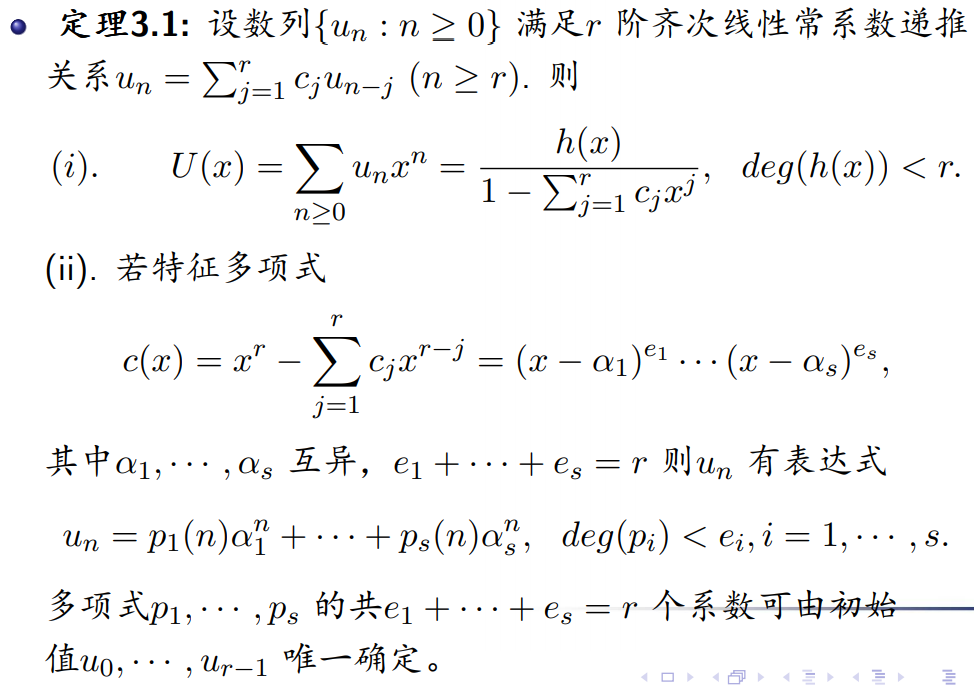
\includegraphics[scale = 0.265]{../src/math/线性齐次线性常系数递推.png}
			
			\subsection{常用生成函数变换}
				$$\frac x {(1 - x) ^ 2} = \sum_{i \ge 0} i x ^ i$$

$$\frac 1 {(1 - x) ^ k} = \sum_{i \ge 0} {i + k - 1 \choose i} x ^ i = \sum_{i \ge 0} {i + k - 1 \choose k - 1}x^i, \; k > 0$$

$$
\begin{aligned}
	\sum_{i = 0} ^ \infty i^n x^i = \sum_{k = 0} ^ n {n \brace k} k! \frac {x^k} {(1-x) ^ {k + 1}} = \sum_{k = 0} ^ n {n \brace k} k! \frac {x^k (1-x) ^ {n – k}} {(1-x) ^ {n + 1}} \\
	= \frac 1 {(1-x) ^ {n + 1}} \sum_{i = 0} ^ n \frac {x^i} {(n-i)!} \sum_{k = 0} ^ i {n \brace k}k!(n-k)! \frac {(-1)^{i-k}} {(i-k)!}
\end{aligned}
$$

(用上面的方法可以把分子化成一个$n$次以内的多项式, 并且可以用一次卷积求出来.)

如果把$i^n$换成任意的一个$n$次多项式, 那么我们可以求出它的下降幂表示形式(或者说是牛顿插值)的系数$r_i$, 发现用$r_k$替换掉上面的${n \brace k}k!$之后其余过程完全相同.

		\newpage
		\section{数论}

			\subsection{$O(n)$ 预处理逆元}
				\inputminted{cpp}{../src/numbertheory/O(n)求逆元.cpp}

			\subsection{线性筛}
				\inputminted{cpp}{../src/numbertheory/扩展线性筛.cpp}

			\subsection{杜教筛}
				$$ S_{\varphi}(n) = \frac {n(n + 1)} 2 - \sum_{d = 2} ^ n S_{\varphi} \left( \left\lfloor \frac n d \right\rfloor \right) $$

$$ S_\mu (n) = 1 - \sum_{d = 2} ^ n S_\mu \left( \left\lfloor \frac n d \right\rfloor \right) $$

\inputminted{cpp}{../src/numbertheory/杜教筛.cpp}
			
			\subsection{Powerful Number 筛}
				注意Powerful Number筛只能求积性函数的前缀和.

本质上就是构造一个方便求前缀和的函数, 然后做类似杜教筛的操作.

定义Powerful Number表示每个质因子幂次都大于$1$的数, 显然最多有$\sqrt n$个.

设我们要求和的函数是$f(n)$, 构造一个方便求前缀和的\textbf{积性}函数$g(n)$使得$g(p) = f(p)$.

那么就存在一个积性函数$h = f * g ^ {-1}$, 也就是$f = g *h$. 可以证明$h(p) = 0$, 所以只有Powerful Number的$h$值不为0.

$$ \begin{aligned}
	S_f(i) = \sum_{d = 1} ^ n h(d) S_g \left( \left\lfloor \frac n d \right\rfloor \right)
\end{aligned} $$

只需要枚举每个Powerful Number作为$d$, 然后用杜教筛计算$g$的前缀和.

求$h(d)$时要先预处理$h(p^k)$, 显然有

$$ \begin{aligned}
	h \left(p ^ k \right) = f \left(p ^ k \right) - \sum_{i = 1} ^ k g \left( p ^ i \right) h \left( p ^ {k - i} \right)
\end{aligned} $$

处理完之后DFS就行了. (显然只需要筛$\sqrt n$以内的质数.)

复杂度取决于杜教筛的复杂度, 特殊题目构造的好也可以做到$O \left( \sqrt n \right)$.

例题:

\begin{itemize}
	\item $f \left( p ^ k \right) = p ^ k \left( p ^ k - 1 \right)$ : $g(n) = \text{id}(n) \varphi(n)$.
	\item $f \left( p ^ k \right) = p \, \text{xor} \, k$ : $n$为偶数时$g(n) = 3 \varphi(n)$, 否则$g(n) = \varphi(n)$.
\end{itemize}

			\subsection{洲阁筛}
				计算积性函数$f(n)$的前$n$项之和时, 我们可以把所有项按照是否有$> \sqrt n$的质因子分两类讨论, 最后将两部分的贡献加起来即可.

~\\

\textbf{1. 有$> \sqrt n$的质因子}

显然$> \sqrt n$的质因子幂次最多为$1$, 所以这一部分的贡献就是

$$ \sum_{i = 1} ^ {\sqrt n} f(i) \sum_{d = \sqrt n + 1} ^ {\left\lfloor \frac n i \right\rfloor} \left[ d \in \mathbb{P} \right] f(d) $$

我们可以DP后面的和式. 由于$f(p)$是一个关于$p$的低次多项式, 我们可以对每个次幂分别DP: 设$g_{i, j}$表示$[1, j]$中和前$i$个质数都互质的数的$k$次方之和. 设$\sqrt n$以内的质数总共有m个, 显然贡献就转换成了

$$ \sum_{i = 1} ^ {\sqrt n} i ^ k g_{m, \left\lfloor \frac n i \right\rfloor} $$

边界显然就是自然数幂次和, 转移是

$$ g_{i, j} = g_{i - 1, j} - p_i ^ k g_{i - 1, \left\lfloor \frac j {p_i} \right\rfloor} $$

也就是减掉和第$i$个质数不互质的贡献.

在滚动数组的基础上再优化一下: 首先如果$j < p_i$那肯定就只有$1$一个数; 如果$p_i \le j < p_i ^ 2$, 显然就有$g_{i, j} = g_{i - 1, j} - p_i ^ k$, 那么对每个$j$记下最大的$i$使得$p_i ^ 2 <= j$, 比这个还大的情况就不需要递推了, 用到的时候再加上一个前缀和解决.

~\\

\textbf{2. z所有质因子都$\le \sqrt n$}

类似的道理, 我们继续DP: $h_{i, j}$表示只含有第$i$到$m$个质数作为质因子的所有数的$f(i)$之和. (这里不需要对每个次幂单独DP了; 另外倒着DP是为了方便卡上限.)

边界显然是$h_{m + 1, j} = 1$, 转移是

$$ h_{i, j} = h_{i + 1, j} + \sum_{c} f(p_i ^ c) h_{i + 1, \left\lfloor \frac j {p_i ^ c} \right\rfloor} $$

跟上面一样的道理优化, 分成三段: $j < p_i$时$h_{i, j} = 1$, $j < p_i ^ 2$时$h_{i, j} = h_{i + 1, j} + f(p_i)$(同样用前缀和解决), 再小的部分就老实递推.

~\\

预处理$\sqrt n$以内的部分之后跑两次DP, 最后把两部分的贡献加起来就行了.

两部分的复杂度都是$\Theta \left( \frac {n ^ {\frac 3 4}} {\log n} \right)$的.

以下代码以洛谷P5325($f(p^k) = p^k (p^k - 1)$)为例.

\inputminted{cpp}{../src/numbertheory/洲阁筛.cpp}

			\subsection{min25 筛}
				假设要求的是

$$ \begin{aligned} \sum_{i = 1} ^ n f(i) \end{aligned} $$

则构造一个函数 $F(n)$, 满足 $F(p) = f(p)$. 注意 $f(p^c)$ 是什么形式是无所谓的.

设 $\sqrt n$ 以内的质数为 $p_1 \dots p_m$, 记

$$ \begin{aligned} g(x) = \sum_{i = 1} ^ x \left[i \in \text{prime}\right] f(i) \end{aligned} $$

$$ \begin{aligned} h(i, n) = \sum_{k = 2} ^ n \left[ k \in \text{prime 或 } k \text{ 与前 } i \text{ 个质数互质} \right] F(k) \end{aligned} $$

显然 $g(x) = h\left( \pi\left(\sqrt x\right), x \right)$.

用递推求出 $h$ 即可. 当 $p_i > \sqrt n$ 时显然有 $h(i, n) = h(i - 1, n)$, 否则有

$$ \begin{aligned} h(i, n) =  h(i - 1, n) - F(p_i) h\left( i - 1, \left\lfloor \frac n {p_i} \right\rfloor \right) + F(p_i) \sum_{k = 1} ^ {i - 1} F(p_k) \end{aligned} $$

边界为 $h(0, n) = \sum_{k = 2} ^ n F(k)$.

设

$$ \begin{aligned} S(i, n) = \sum_{k = 2} ^ n \left[ k \text{ 与前 } i \text{ 个质数互质} \right] f(k) \end{aligned}$$

则

$$ \begin{aligned} S(i, n) = g(n) - \sum_{k = 1} ^ {i - 1} f(p_k) + \end{aligned} $$
$$ \begin{aligned} \sum_{k = i} ^ {p_k \le \sqrt n} \sum_{c = 1} ^ {p_k ^ {c + 1} \le n} S\left( k + 1, \left\lfloor \frac n {p_k ^ c} \right\rfloor \right) f\left( p_k ^ c \right) + f\left( p_k ^ {c + 1} \right) \end{aligned} $$

这里直接递归即可, 最后的答案即为 $\text{ans} = S(1, n) + f(1)$.

			% \subsection{离散对数(BSGS)(待完成)}

			\subsection{Miller-Rabin}
				\inputminted{cpp}{../src/numbertheory/Miller-Rabin.cpp}

			\subsection{Pollard's Rho}
				\inputminted{cpp}{../src/numbertheory/Pollard-Rho.cpp}
			
			\subsection{快速阶乘算法}
				参见\ref{fastfact}.\nameref{fastfact} (第 \pageref{fastfact} 页).

			% \subsection{组合数取模}


			\subsection{扩展欧几里德 exgcd}
				\inputminted{cpp}{../src/numbertheory/exgcd.cpp}
				\subsubsection{求通解的方法}

假设我们已经找到了一组解$(p_0, q_0)$满足$a p_0 + b q_0 = \gcd(a,b)$, 那么其他的解都满足

$$p = p_0 + \frac b {\gcd(p, q)} \times t\quad\quad q = q_0 - \frac a {\gcd(p, q)} \times t$$

其中t为任意整数.

				\subsubsection{类欧几里德算法(直线下整点个数)}
					$a,b \ge 0, m > 0$, 计算$\sum_{i = 0} ^ {n - 1} \left\lfloor \frac {a + bi} m \right\rfloor$.
					\inputminted{cpp}{../src/numbertheory/类欧.cpp}
			
			\subsection{中国剩余定理}
				$$ x \equiv a_i \pmod {m_i} $$

$$ M = \prod_i m_i,\; M_i = \frac M {m_i} $$

$$ M_i' \equiv M_i^{-1} \pmod {m_i} $$

$$ x \equiv \sum_{i} a_i M_i M_i' \pmod M $$

				\subsubsection{ex-CRT}
					设两个方程分别是 $x\equiv a_1 \pmod {m_1}$ 和 $x\equiv a_2 \pmod {m_2}$。

将它们转化为不定方程 $x = m_1 p + a_1 = m_2 q + a_2$,其中 $p, q$ 是整数,则有 $m_1 p - m_2 q = a_2 - a_1$。

当 $a_2 - a_1$ 不能被 $\gcd(m_1, m_2)$ 整除时无解,否则可以通过扩展欧几里德解出来一组可行解 $(p, q)$。

则原来的两方程组成的模方程组的解为 $x\equiv b\pmod M$,其中 $b = m_1 p + a_1$,$M = \text{lcm}(m_1, m_2)$。

			
			\subsection{二次剩余}
				\inputminted{cpp}{../src/numbertheory/二次剩余.cpp}
			
			% \subsection{组合数取模(ex-Lucas)(待完成)}
			
			\subsection{原根 阶}
				\textbf{阶}: 最小的整数$k$使得$a ^ k \equiv 1 \pmod p$, 记为$\delta_p(a)$.

显然$a$在原根以下的幂次是两两不同的.

一个性质: 如果$a, b$均与$p$互质, 则 $ \delta_p(ab)=\delta_p(a)\delta_p(b) $ 的充分必要条件是$ \gcd\big(\delta_p(a),\delta_p(b)\big)=1 $.

另外, 如果$a$与$p$互质, 则有$ \delta_p(a^k)=\dfrac{\delta_p(a)}{\gcd\big(\delta_p(a),k\big)} $. (也就是环上一次跳$k$步的周期.)

\textbf{原根}: 阶等于$\varphi(p)$的数.

只有形如$2, 4, p ^ k, 2 p ^ k$($p$是奇素数)的数才有原根, 并且如果一个数$n$有原根, 那么原根的个数是$\varphi(\varphi(n))$个.

暴力找原根代码:
\begin{minted}{python}
def split(n): # 分解质因数
    i = 2
    a = []
    while i * i <= n:
        if n % i == 0:
            a.append(i)

            while n % i == 0:
                n /= i

        i += 1

    if n > 1:
        a.append(n)

    return a
    
def getg(p): # 找原根
    def judge(g):
        for i in d:
            if pow(g, (p - 1) / i, p) == 1:
                return False
        return True

    d = split(p - 1)
    g = 2

    while not judge(g):
        g += 1

    return g

print(getg(int(input())))
\end{minted}
			
			\subsection{常用数论公式}
				\subsubsection{莫比乌斯反演}
	$$ \begin{aligned}
		f(n) = \sum_{d | n} g(d) \Leftrightarrow g(n) = \sum_{d | n} \mu\left( \frac n d \right) f(d) \\
		f(d) = \sum_{d | k} g(k) \Leftrightarrow g(d) = \sum_{d | k} \mu\left( \frac k d \right) f(k)
	\end{aligned} $$

\subsubsection{降幂公式}

$$ a^k \equiv a ^ {k \bmod \varphi(p) + \varphi(p)},\; k \ge \varphi(p) $$

\subsubsection{其他常用公式}
	$$\mu * I = e \quad (e(n) = [n = 1])$$

	$$\varphi * I = id $$

	$$\mu * id = \varphi $$

	$$\sigma_0 = I * I ,\, \sigma_1 = id * I ,\, \sigma_k = id^{k - 1} * I$$

	$$\sum_{i = 1} ^ n \left[(i, n) = 1\right] i = n \frac {\varphi(n) + e(n)} 2$$
	
	$$\sum_{i = 1} ^ n \sum_{j = 1} ^ i \left[(i, j) = d\right] = S_\varphi \left( \left\lfloor \frac n d \right\rfloor \right)$$

	$$\sum_{i = 1} ^ n \sum_{j = 1} ^ m \left[(i, j) = d\right] = \sum_{d | k} \mu\left( \frac k d \right) \left\lfloor \frac n k \right\rfloor \left\lfloor \frac m k \right\rfloor$$

	$$ \sum_{i = 1} ^ n f(i) \sum_{j = 1} ^ {\left\lfloor \frac n i \right\rfloor} g(j) = \sum_{i = 1} ^ n g(i) \sum_{j = 1} ^ {\left\lfloor \frac n i \right\rfloor} f(j) $$
				
		\newpage
		\section{图论}

			\subsection{最小生成树}
				\subsubsection{Boruvka 算法}
					思想: 每次选择连接每个连通块的最小边, 把连通块缩起来. \\
每次连通块个数至少减半, 所以迭代$O(\log n)$次即可得到最小生成树.

一种比较简单的实现方法: 每次迭代遍历所有边, 用并查集维护连通性和每个连通块的最小边权.

应用: 最小异或生成树
				
				\subsubsection{动态最小生成树}
					动态最小生成树的离线算法比较容易, 而在线算法通常极为复杂.

一个跑得比较快的离线做法是对时间分治, 在每层分治时找出一定在/不在MST上的边, 只带着不确定边继续递归.

简单起见, 找确定边的过程用Kruskal算法实现, 过程中的两种重要操作如下:

\begin{itemize}
	\item Reduction: 待修改边标为$+\infty$, 跑MST后把非树边删掉, 减少无用边
	\item Contraction: 待修改边标为$-\infty$, 跑MST后缩除待修改边之外的所有MST边, 计算必须边
\end{itemize}

每轮分治需要Reduction-Contraction, 借此减少不确定边, 从而保证复杂度.

复杂度证明: 假设当前区间有$k$条待修改边, $n$和$m$表示点数和边数, 那么最坏情况下R-C的效果为$(n, m) \to (n, n + k - 1) \to (k + 1, 2k)$.

\inputminted{cpp}{../src/graph/动态最小生成树.cpp}
				
				\subsubsection{最小树形图}
					对每个点找出最小的入边, 如果是一个DAG那么就已经结束了.

否则把环都缩起来再跑一遍, 直到没有环为止.

可以用可并堆优化到$O(m\log n)$, 需要写一个带懒标记的左偏树.
				
				\subsubsection{Steiner Tree 斯坦纳树}
					\paragraph{问题} 一张图上有 $k$ 个关键点,求让关键点两两连通的最小生成树。

\paragraph{做法} 状压 DP,$f_{i,S}$ 表示以 $i$ 号点为树根,$i$ 与 $S$ 中的所有点连通的最小边权和。

转移有两种:

\begin{enumerate}
	\item 枚举子集:
	$$ f_{i, S} = \min_{T\subset S} \left\{f_{i, T} + f_{i, S\setminus T}\right\} $$
	\item 新加一条边: 
	$$ f_{i, S} = \min_{(i, j)\in E} \left\{f_{j, S} + w_{i, j}\right\} $$
\end{enumerate}

第一种直接枚举子集 DP 就行了,第二种可以用 SPFA 或者 Dijkstra 松弛(显然负边一开始全选就行了,所以只需要处理非负边)。

复杂度 $O(n 3^k + 2^k \text{SSSP}(n, m)))$,其中 $\text{SSSP}(n,m)$ 可以是 $nm$(SPFA)或者 $n^2+m$ 或者 $m\log n$(后两种都是 Dijkstra)。

\inputminted{cpp}{../src/graph/steiner.cpp}

				
				\subsubsection{最小直径生成树}
					首先要找到图的绝对中心(可能在点上, 也可能在某条边上), 然后以绝对中心为起点建最短路树就是最小直径生成树.

\inputminted{cpp}{../src/graph/mdst.cpp}
			
			\subsection{最短路}
				\subsubsection{Dijkstra}
					参见\ref{kshortestpath}.\nameref{kshortestpath}(第 \pageref{kshortestpath} 页), 注意那边是求到$t$的最短路.
				
				\subsubsection{Johnson 算法(负权图多源最短路)}
					首先前提是图没有负环.

先任选一个起点$s$, 跑一边SPFA, 计算每个点的势$h_u = d_{s, u}$, 然后将每条边$u\to v$的权值$w$修改为$w + h[u] - h[v]$即可, 由最短路的性质显然修改后边权非负.

然后对每个起点跑Dijkstra, 再修正距离$d_{u, v} = d'_{u, v} - h_u + h_v$即可, 复杂度$O(nm\log n)$, 在稀疏图上是要优于Floyd的.
				
				% \subsubsection{差分约束}


				\subsubsection{$k$短路}
					\label{kshortestpath}
					\inputminted{cpp}{../src/graph/k短路.cpp}
			
			\subsection{Tarjan 算法}
				\subsubsection{强连通分量}
					\inputminted{cpp}{../src/graph/强连通分量.cpp}
				
				\subsubsection{割点 点双}
					\inputminted{cpp}{../src/graph/割点点双.cpp}

				\subsubsection{桥 边双}
					\inputminted{cpp}{../src/graph/边双.cpp}
			
			\subsection{欧拉回路}
				\mintinline{cpp}{C[x]}是记录每条边对应的编号的.
				
				另外为了保证复杂度需要加当前弧优化.
				
				\inputminted{cpp}{../src/graph/欧拉回路.cpp}

			\subsection{仙人掌}
				一般来说仙人掌问题都可以通过圆方树转成有两种点的树上问题来做.
				\subsubsection{仙人掌 DP}
					\inputminted{cpp}{../src/graph/仙人掌DP.cpp}
			
			\subsection{二分图}
				\subsubsection{匈牙利}
					\inputminted{cpp}{../src/graph/hungary.cpp}

				\subsubsection{Hopcroft-Karp 二分图匹配}
					其实长得和 Dinic 差不太多, 或者说像匈牙利和 Dinic 的缝合怪.
					\inputminted{cpp}{../src/graph/hopcroft-karp.cpp}

				\subsubsection{KM 二分图最大权匹配}
					\inputminted{cpp}{../src/graph/KM二分图最大权匹配.cpp}

				\subsubsection{二分图原理}
					\textbf{最大匹配的可行边与必须边, 关键点}

以下的``残量网络''指网络流图的残量网络.

\begin{itemize}
	\item 可行边: 一条边的两个端点在残量网络中处于同一个SCC, 不论是正向边还是反向边.

	\item 必须边: 一条属于当前最大匹配的边, 且残量网络中两个端点不在同一个SCC中.
	
	\item 关键点(必须点): 这里不考虑网络流图而只考虑原始的图, 将匹配边改成从右到左之后从左边的每个未匹配点进行floodfill, 左边没有被标记的点即为关键点. 右边同理.
\end{itemize}

\textbf{独立集}

二分图独立集可以看成最小割问题, 割掉最少的点使得S和T不连通, 则剩下的点自然都在独立集中.

所以独立集输出方案就是求出不在最小割中的点, 独立集的必须点/可行点就是最小割的不可行点/非必须点.

割点等价于割掉它与源点或汇点相连的边, 可以通过设置中间的边权为无穷以保证不能割掉中间的边, 然后按照上面的方法判断即可.

(由于一个点最多流出一个流量, 所以中间的边权其实是可以任取的.)

\textbf{二分图最大权匹配}

二分图最大权匹配的对偶问题是最小顶标和问题, 即: 为图中的每个顶点赋予一个非负顶标, 使得对于任意一条边, 两端点的顶标和都要不小于边权, 最小化顶标之和.

显然KM算法的原理实际上就是求最小顶标和.
			
			\subsection{一般图匹配}
				\subsubsection{高斯消元}
					\inputminted{cpp}{../src/graph/基于线性代数的一般图匹配.cpp}

				\subsubsection{带花树}
					\inputminted{cpp}{../src/graph/带花树.cpp}
				
				\subsubsection{带权带花树}
					Forked from the template of Imperisible Night.

					(有一说一这玩意实在太难写了, 抄之前建议先想想算法是不是假的或者有SB做法)
					\inputminted{cpp}{../src/graph/带权带花树.cpp}
				
				\subsubsection{原理}
					设图$G$的Tutte矩阵是$\tilde A$, 首先是最基础的引理:

\begin{itemize}
	\item $G$的最大匹配大小是$\frac 1 2 \text{rank}{\tilde A}$.
	
	\item $({\tilde A} ^{-1}) _{i, j} \ne 0$当且仅当$G-\{v_i, v_j\}$有完美匹配.
		\subitem (考虑到逆矩阵与伴随矩阵的关系, 这是显然的.)
\end{itemize}

构造最大匹配的方法见板子. 对于更一般的问题, 可以借助构造方法转化为完美匹配问题.

设最大匹配的大小为$k$, 新建$n - 2 k$个辅助点, 让它们和其他所有点连边, 那么如果一个点匹配了一个辅助点, 就说明它在原图的匹配中不匹配任何点.

\begin{itemize}
	\item 最大匹配的可行边: 对原图中的任意一条边$(u, v)$, 如果删掉$u, v$后新图仍然有完美匹配(也就是${\tilde A} ^ {-1}_{u, v} \ne 0$), 则它是一条可行边.
	
	\item 最大匹配的必须边: \textbf{待补充}
	
	\item 最大匹配的必须点: 可以删掉这个点和一个辅助点, 然后判断剩下的图是否还有完美匹配, 如果有则说明它不是必须的, 否则是必须的. 只需要用到逆矩阵即可.
	
	\item 最大匹配的可行点: 显然对于任意一个点, 只要它不是孤立点, 就是可行点.
\end{itemize}

			
			\subsection{支配树}
				\textbf{记得建反图!}
				\inputminted{cpp}{../src/graph/支配树.cpp}

			\subsection{2-SAT}
				如果限制满足对称性(每个命题的逆否命题对应的边也存在), 那么可以使用Tarjan算法求SCC搞定. 

具体来说就是, 如果某个变量的两个点在同一SCC中则显然无解, 否则按拓扑序倒序尝试选择每个SCC即可.

由于Tarjan算法的特性, 找到SCC的顺序就是拓扑序\textbf{倒序}, 所以判断完是否有解之后, 每个变量只需要取SCC编号\textbf{较小}的那个.

\inputminted{cpp}{../src/graph/2sat-tarjan.cpp}

如果要字典序最小就用DFS, 注意可以压位优化. 另外代码是0-base的.

\inputminted{cpp}{../src/graph/2sat.cpp}

			\subsection{最大流}
				\subsubsection{Dinic}
					\inputminted{cpp}{../src/graph/Dinic.cpp}

				\subsubsection{ISAP}
					\textbf{可能有毒, 慎用.}
					\inputminted{cpp}{../src/graph/ISAP.cpp}

				\subsubsection{HLPP 最高标号预流推进}
					\inputminted{cpp}{../src/graph/HLPP.cpp}
			
			\subsection{费用流}
				\subsubsection{SPFA 费用流}
					\inputminted{cpp}{../src/graph/SPFA费用流.cpp}

				\subsubsection{Dijkstra 费用流}
					有的地方也叫原始-对偶费用流.

原理和求多源最短路的Johnson算法是一样的, 都是给每个点维护一个势$h_u$, 使得对任何有向边$u\to v$都满足$w + h_u - h_v \ge 0$.

如果有负费用则从$s$开始跑一遍SPFA初始化, 否则可以直接初始化$h_u = 0$.

每次增广时得到的路径长度就是$d_{s, t} + h_t$, 增广之后让所有$h_u = h'_u + d'_{s, u}$, 直到$d_{s, t} = \infty$(最小费用最大流)或$d_{s, t} \ge 0$(最小费用流)为止.

注意最大费用流要转成取负之后的最小费用流, 因为Dijkstra求的是最短路.

\inputminted{cpp}{../src/graph/dijkstra费用流.cpp}
				
				\subsubsection{预流推进费用流(可处理负环) $O(nm \log C)$}
					不是很懂什么原理, 待研究.

					\inputminted{cpp}{../src/graph/预流推进费用流.cpp}

				% \subsubsection{zkw费用流}


				% \subsubsection{网络单纯形}
			

			\subsection{网络流原理}
				\subsubsection{最大流}

\begin{itemize}

\item \textbf{判断一条边是否必定满流}

在残量网络中跑一遍 Tarjan,如果某条满流边的两端处于同一 SCC 中,则说明它不一定满流。(因为可以找出包含反向边的环,增广之后就不满流了。)

\end{itemize}

\subsubsection{最小割}

首先牢记最小割的定义:选权值和尽量小的一些边,使得删除这些边之后 $s$ 无法到达 $t$。

\paragraph{最小割输出一种方案}
在残量网络上从 $S$ 开始 floodfill,源点可达的记为 $S$ 集,不可达的记为 $T$ 集。如果一条边的起点在 $S$ 集而终点在 $T$ 集,就将其加入最小割中。

\paragraph{最小割的可行边与必须边}
\begin{itemize}
	\item 可行边: 满流,且残量网络上不存在 $u$ 到 $v$ 的路径,也就是 $u$ 和 $v$ 不在同一 SCC 中。(实际上也就是最大流必定满流的边。)

	\item 必须边:满流,且残量网络上 $S$ 可达 $u$,$v$ 可达 $T$。
\end{itemize}

\paragraph{字典序最小的最小割}
直接按字典序从小到大的顺序依次判断每条边能否在最小割中即可。

如果一条边是可行边,我们就需要把它删掉,同时进行退流,$u\to s$ 和 $t\to v$都 退掉等同于这条边容量的流量。

退流用 Dinic 实现即可。

% \subsubsection{费用流}


\subsubsection{上下界网络流}

\paragraph{无源汇上下界可行流}
新建源汇 $S', T'$,然后如图所示转化每一条边。

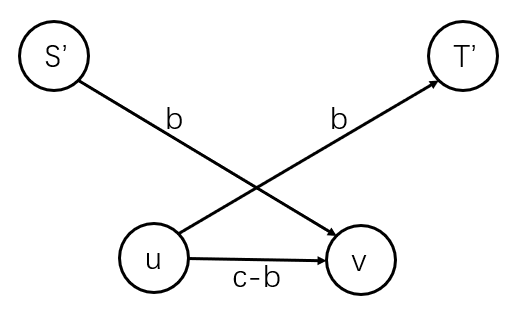
\includegraphics[scale = 0.5]{../src/graph/上下界网络流.png}

在新图跑一遍最大流之后检查一遍辅助边,如果有辅助边没满流则无解,否则把每条边的流量加上 $b$ 就是一组可行方案。

\paragraph{有源汇上下界最大流}
如果不需要判断是否有解的话,可以直接按照和上面一样的方法转化。因为附加边实际上算了两次流量,所以最终答案应该减掉所有下界之和。

(另外这里如果要压缩附加边的话,不能像无源汇的情况一样对每个点只开一个变量统计溢出的流量。正确的做法是进出流量各统计一下,每个点连两条附加边。)

如果需要判有解的话会出一点问题。这时候就需要转化成无源汇的情况,验证有解之后撤掉 $T$ 到 $S$ 的那条附加边,再从 $S$ 到 $T$ 跑一遍最大流。

\inputminted{cpp}{../src/graph/有源汇上下界最大流.cpp}

\paragraph{有源汇上下界最小流}
按照上面的方法转换后先跑一遍最大流,然后撤掉超级源汇和附加边,反过来跑一次最大流退流,最大流减去退掉的流量就是最小流。

\subsubsection{常见建图方法}

\begin{itemize}

\item \textbf{最大流/费用流}

流量不是很多的时候可以理解成很多条路径,并且每条边可以经过的次数有限。

\item \textbf{最小割}

常用的模型是 \textbf{最大权闭合子图}。当然它并不是万能的,因为限制条件可以带权值。

\begin{enumerate}

\item 如果某些点全部在 $S$ 集或者 $T$ 集,则获得一个正的收益

把这个条件建成一个点,向要求的点连 $+\infty$ 边,然后 $s$ 向它连 $+\infty$ 边。(如果是 $T$ 集就都反过来)

那么如果它在 $S$ 集,就一定满足它要求的点都在 $S$ 集,反之如果是 $T$ 集亦然。

\item 如果两个点不在同一集合中,则需要付出代价

建双向边,那显然如果它们不在同一集合中就需要割掉中间的边,付出对应的代价。

\item 二分图,如果相邻的两个点在同一集合则需要付出代价

染色后给一半的点反转源汇,就转换成上面的问题了。

\end{enumerate}

\end{itemize}

\subsubsection{例题}

\begin{itemize}

% \item 最大流



% \item 最小割

% \begin{enumerate}

% \item 切糕

% \end{enumerate}

\item 费用流

\begin{enumerate}

\item 序列上选总和尽量大的数,但连续 $k$ 个数中最多选 $p$ 个

费用流建图,先建一条 $n+1$ 个点的无限容量的链表示不选,然后每个 $i$ 向 $(i + k)$ 连边费用是第 $i$ 个位置的权值。答案是流量为 $p$ 的最大费用流,因为条件等价于选 $p$ 次并且每次选的所有数间隔都至少是 $k$。

\item 除此之外还要求连续 $k$ 个数中最少选 $q$ 个

任选一个位置把图前后切开,会发现通过截面的流量总和恰为 $p$。注意到如果走了最开始的链就代表不选,因此要限制至少有 $q$
的流量不走链,那么只需要把链的容量改成 $p - q$ 就行了。

\end{enumerate}

\end{itemize}

			
			\subsection{Prufer序列}
				对一棵有$n \ge 2$个结点的树, 它的Prufer编码是一个长为$n - 2$, 且每个数都在$[1, n]$内的序列.

构造方法: 每次选取编号最小的叶子结点, 记录它的父亲, 然后把它删掉, 直到只剩两个点为止. (并且最后剩的两个点一定有一个是$n$号点.)

相应的, 由Prufer编码重构树的方法: 按顺序读入序列, 每次选取编号最小的且度数为$1$的结点, 把这个点和序列当前点连上, 然后两个点剩余度数同时$-1$. 

\large\textbf{Prufer编码的性质}

\begin{itemize}
	\item 每个至少$2$个结点的树都唯一对应一个Prufer编码. (当然也就可以做无根树哈希.)
	\item 每个点在Prufer序列中出现的次数恰好是度数$-1$. 所以如果给定某些点的度数然后求方案数, 就可以用简单的组合数解决.
\end{itemize}


最后, 构造和重构直接写都是$O(n\log n)$的, 想优化成线性需要一些技巧.

线性求Prufer序列代码:
\begin{minted}{cpp}
// 0-based
vector<vector<int>> adj;
vector<int> parent;

void dfs(int v) {
  for (int u : adj[v]) {
    if (u != parent[v]) parent[u] = v, dfs(u);
  }
}

vector<int> pruefer_code() { // pruefer是德语
  int n = adj.size();
  parent.resize(n), parent[n - 1] = -1;
  dfs(n - 1);

  int ptr = -1;
  vector<int> degree(n);
  for (int i = 0; i < n; i++) {
    degree[i] = adj[i].size();
    if (degree[i] == 1 && ptr == -1) ptr = i;
  }

  vector<int> code(n - 2);
  int leaf = ptr;
  for (int i = 0; i < n - 2; i++) {
    int next = parent[leaf];
    code[i] = next;
    if (--degree[next] == 1 && next < ptr) {
      leaf = next;
    } else {
      ptr++;
      while (degree[ptr] != 1) ptr++;
      leaf = ptr;
    }
  }
  return code;
}
\end{minted}

线性重构树代码:
\begin{minted}{cpp}
// 0-based
vector<pair<int, int>> pruefer_decode(vector<int> const& code) {
	int n = code.size() + 2;
	vector<int> degree(n, 1);
	for (int i : code) degree[i]++;

	int ptr = 0;
	while (degree[ptr] != 1) ptr++;
	int leaf = ptr;

	vector<pair<int, int>> edges;
	for (int v : code) {
	edges.emplace_back(leaf, v);
	if (--degree[v] == 1 && v < ptr) {
		leaf = v;
	} else {
		ptr++;
		while (degree[ptr] != 1) ptr++;
		leaf = ptr;
	}
	}
	edges.emplace_back(leaf, n - 1);
	return edges;
}
\end{minted}

			\subsection{弦图相关}
				Forked from the template of NEW CODE!!.
				\begin{enumerate}
	\item 团数 $\leq$ 色数,弦图团数 = 色数;
	
	\item 设 $next(v)$ 表示 $N(v)$ 中最前的点,
	令 $w*$ 表示所有满足 $A \in B$ 的 $w$ 中最后的一个点,判断 $v \cup N(v)$ 是否为极大团,
	只需判断是否存在一个 $w$,满足 $Next(w)=v$ 且 $|N(v)| + 1 \leq |N(w)|$ 即可。
	
	\item 最小染色:完美消除序列 \textbf{从后往前}\ 依次给每个点染色,给每个点染上可以染的最小的颜色。
	
	\item 最大独立集:完美消除序列 \textbf{从前往后}\ 能选就选。
	
	\item 弦图最大独立集数 $=$ 最小团覆盖数。
	
	\item 最小团覆盖:设最大独立集为 $\{p_1,p_2, \dots ,p_t\}$,
	则 $\{p_1\cup N(p_1), \dots , p_t \cup N(p_t)\}$  为最小团覆盖。
\end{enumerate}


			% \subsection{弦图}
				% \subsubsection{完美消除序列, 最大势算法}


				% \subsubsection{性质}
			

			\subsection{其他}
				\subsubsection{Stoer-Wagner 全局最小割}
					\inputminted{cpp}{../src/graph/stoer-wagner.cpp}

				% \subsubsection{最小割树}


				% \subsubsection{最大团搜索}
			
		\newpage
		\section{数据结构}

			\subsection{线段树}
				\subsubsection{非递归线段树}
					% \sout{让fstqwq手撕}

\begin{itemize}
	\item 如果$M = 2^k$, 则只能维护$[1, M - 2]$范围
	\item 找叶子: $i$对应的叶子就是$i + M$
	\item 单点修改: 找到叶子然后向上跳
	\item 区间查询: 左右区间各扩展一位, 转换成开区间查询
	\inputminted{cpp}{../src/datastructure/非递归线段树单点修改.cpp}

\end{itemize}
	
区间修改要标记永久化,并且求区间和和求最值的代码不太一样. \\

\textbf{区间加, 区间求和}
\inputminted{cpp}{../src/datastructure/非递归线段树区间加区间求和.cpp}

\textbf{区间加, 区间求最大值}
\inputminted{cpp}{../src/datastructure/非递归线段树区间加区间求最大值.cpp}
				
				\subsubsection{线段树维护矩形并}
					为线段树的每个结点维护 $cover_i$ 表示这个区间被完全覆盖的次数.

					更新时分情况讨论, 如果当前区间已被完全覆盖则长度就是区间长度, 否则长度是左右儿子相加.
					\inputminted{cpp}{../src/datastructure/线段树维护矩形并.cpp}
				
				\subsubsection{历史和}

					EC-Final2020 G, 原题是询问某个区间有多少子区间, 满足子区间中数的种类数为奇数.

					离线之后转化成枚举右端点并用线段树维护左端点, 然后就是一个支持区间反转 (0/1 互换) 和询问历史和的线段树.

					``既然标记会复合,就说明在两个标记中间没有经过任何 pushup 操作

					也就是说一个这两个标记对应着 相同的 0 的数量 以及 相同的 1 的数量

					那么标记对于答案的影响只能是 a * 0 + b * 1

					我们维护 a,b 即可''

					\inputminted{cpp}{../src/datastructure/ec20g.cpp}

				% \subsubsection{主席树离线求区间mex(待完成)}
					
	
			\subsection{陈丹琦分治}
				\subsubsection{动态图连通性 (分治并查集)}
					\inputminted{cpp}{../src/datastructure/分治并查集.cpp}

				\subsubsection{四维偏序}
					\inputminted{cpp}{../src/datastructure/CDQ分治.cpp}
	
			\subsection{整体二分}
				修改和询问都要划分, 备份一下, 递归之前copy回去.

				如果是满足可减性的问题(例如查询区间 $k$ 小数)可以直接在划分的时候把询问的 $k$ 修改一下. 否则需要维护一个全局的数据结构, 一般来说可以先递归右边再递归左边, 具体维护方法视情况而定.

				以下代码以ZJOI K大数查询为例(区间都添加一个数, 询问区间 $k$ 大数).

				\inputminted{cpp}{../src/datastructure/整体二分.cpp}

			% \subsection{块状链表}
	
	
			\subsection{平衡树}
				pb\_ds 平衡树参见 \ref{pbds}.\nameref{pbds} (第 \pageref{pbds} 页).

				\subsubsection{Treap}
					\inputminted{cpp}{../src/datastructure/Treap.cpp}
					
				\subsubsection{无旋 Treap / 可持久化 Treap}
					\inputminted{cpp}{../src/datastructure/无旋Treap.cpp}
		
				\subsubsection{Splay}
					如果插入的话可以直接找到底然后 splay 一下, 也可以直接 splay 前驱后继.
					\inputminted{cpp}{../src/datastructure/文艺平衡树.cpp}
				
			\subsection{树链剖分}
				\subsubsection{动态树形 DP (最大权独立集)}
					\inputminted{cpp}{../src/datastructure/动态树形DP.cpp}
				
			\subsection{树分治}
				% \subsubsection{静态树分治}

				
				\subsubsection{动态树分治}
					\inputminted{cpp}{../src/datastructure/动态树分治.cpp}

				\subsubsection{紫荆花之恋}
					稍微重构了一下, 修改了代码风格.

					另外这个是BFS版本, 跑得比DFS要快不少. (虽然主要复杂度并不在重构上)
					\inputminted{cpp}{../src/datastructure/紫荆花之恋.cpp}
	
			\subsection{LCT动态树}
				\subsubsection{不换根(弹飞绵羊)}
					\inputminted{cpp}{../src/datastructure/LCT(不换根).cpp}
			
				\subsubsection{换根/维护生成树}
					\inputminted{cpp}{../src/datastructure/LCT(换根).cpp}

				\subsubsection{维护子树信息}
					\inputminted{cpp}{../src/datastructure/LCT维护子树信息.cpp}
					
				\subsubsection[模板题:动态QTREE4]{模板题:动态 QTREE4 (询问树上相距最远点)}
						\inputminted{cpp}{../src/datastructure/动态QTREE4.cpp}
	
			\subsection{K-D树}

				\subsubsection{动态 K-D 树(定期重构)}
					\inputminted{cpp}{../src/datastructure/动态KD树.cpp}
	
			% \subsection{树分块}
	
	
			% \subsection{树上莫队}
			
			\subsection{LCA 最近公共祖先}
				\subsubsection{Tarjan LCA $O(n + m)$}
					\inputminted{cpp}{../src/datastructure/tarjanlca.cpp}

			\subsection{虚树}
				\inputminted{cpp}{../src/datastructure/虚树.cpp}
	
			\subsection{长链剖分}
				\inputminted{cpp}{../src/datastructure/长链剖分.cpp}
	
				\subsubsection{梯子剖分}
					\inputminted{cpp}{../src/datastructure/梯子剖分.cpp}
			
			\subsection{堆}

				\subsubsection{左偏树}
					参见\ref{kshortestpath}.k短路 (第 \pageref{kshortestpath} 页).
				
				\subsubsection{二叉堆}
					\inputminted{cpp}{../src/datastructure/二叉堆.cpp}
			
			\subsection{莫队}
				注意如果$n$和$q$不平衡, 块大小应该设为$\frac n {\sqrt q}$.

另外如果裸的莫队要卡常可以按块编号奇偶性分别对右端点正序或者倒序排序, 期望可以减少一半的移动次数.


\subsubsection{回滚莫队(无删除莫队)(待完成)}

\subsubsection{莫队二次离线}

适用范围: 询问的是点对相关(或者其它可以枚举每个点和区间算贡献)的信息, 并且可以离线; 更新时可以使用一些牺牲修改复杂度来改善询问复杂度的数据结构(如单点修改询问区间和).

先按照普通的莫队将区间排序. 考虑区间移动的情况, 以$(l, r)$向右移动右端点到$(l, t)$为例.

对于每个$i \in (r, t]$来说, 它都要对区间$[l, i)$算贡献. 可以拆成$[1, i)$和$[1, l)$两部分, 那么前一部分因为都是$i$和$[1, i)$做贡献的形式所以可以直接预处理.

考虑后一部分, $i$和$(1, l]$做贡献, 因为莫队的性质我们可以保证这样的询问次数不超过$O((n + m)\sqrt n)$, 因此我们可以对每个$l$记录下来哪些$i$要和它询问. 并且每次移动时询问的$i$都是连续的, 所以对每个$l$开一个vector记录下对应的区间和编号就行了.

剩余的三种情况(右端点左移或者移动左端点)都是类似的, 具体可以看代码.

例: Yuno loves sqrt technology II (询问区间逆序对数)

\inputminted{cpp}{../src/datastructure/莫队二次离线.cpp}

\subsubsection{带修莫队在线化 $O(n ^ {\frac 5 3})$}

最简单的带修莫队: 块大小设成$n^{\frac 2 3}$, 排序时第一关键字是左端点块编号, 第二关键字是右端点块编号, 第三关键字是时间. (记得把时间压缩成只有修改的时间.)

现在要求在线的同时支持修改, 仍然以$B = n^{\frac 2 3}$分一块, 预处理出两块之间的贡献, 那么预处理复杂度就是$O(n ^ {\frac 5 3})$.

修改时最简单的方法是直接把$n^{\frac 2 3}$个区间全更新一遍. 嫌慢的话可以给每个区间打一个懒标记, 询问的时候如果解了再更新区间的信息.

注意如果附加信息是可减的(比如每个数的出现次数), 那么就只需要存$O(n^{\frac 1 3})$个.

总复杂度仍然是$O(n^{\frac 5 3})$, 如果打懒标记的话是跑不太满的. 如果附加信息可减则空间复杂度是$O(n^{\frac 4 3})$, 否则和时间复杂度同阶.

\subsubsection{莫队二次离线 在线化 $O((n + m)\sqrt n)$}

和之前的道理是一样的, $i$和$[1, i)$的贡献这部分仍然可以预处理掉, 而前后缀对区间的贡献那部分只保存块端点处的信息.

按照莫队二次离线的转移方法操作之后发现只剩两边散块的贡献没有解决. 这时可以具体问题具体解决, 例如求逆序对的话直接预处理出排序后的数组然后归并即可.

时空复杂度均为$O(n\sqrt n)$.

以下代码以强制在线求区间逆序对为例(洛谷上被卡常了, 正常情况下极限数据应该在1.5s内.)

\inputminted{cpp}{../src/datastructure/莫队二次离线在线化.cpp}
	
			\subsection{常见根号思路}
				
\noindent{
	{\large\bfseries{通用}}
	\begin{itemize}
		\item 出现次数大于$\sqrt n$的数不会超过$\sqrt n$个
		\item 对于带修改问题, 如果不方便分治或者二进制分组, 可以考虑对操作分块, 每次查询时暴力最后的$\sqrt n$个修改并更正答案
		\item {\bfseries 根号分治}: 如果分治时每个子问题需要$O(N)$(N是全局问题的大小)的时间, 而规模较小的子问题可以$O(n^2)$解决, 则可以使用根号分治
			\begin{itemize}
				\item 规模大于$\sqrt n$的子问题用$O(N)$的方法解决, 规模小于$\sqrt n$的子问题用$O(n^2)$暴力
				\item 规模大于$\sqrt n$的子问题最多只有$\sqrt n$个
				\item 规模不大于$\sqrt n$的子问题大小的平方和也必定不会超过$n\sqrt n$
			\end{itemize}
		\item 如果输入规模之和不大于$n$(例如给定多个小字符串与大字符串进行询问), 那么规模超过$\sqrt n$的问题最多只有$\sqrt n$个
	\end{itemize}
}

\noindent{
	{\large\bfseries{序列}}
	\begin{itemize}
		\item 某些维护序列的问题可以用分块/块状链表维护
		\item 对于静态区间询问问题, 如果可以快速将左/右端点移动一位, 可以考虑莫队
			\begin{itemize}
				\item 如果强制在线可以分块预处理, 但是一般空间需要$n\sqrt n$ 
					\begin{itemize}
						\item 例题: 询问区间中有几种数出现次数恰好为$k$, 强制在线
					\end{itemize}
				\item 如果带修改可以试着想一想带修莫队, 但是复杂度高达$n^{\frac 5 3}$
			\end{itemize}
		\item 线段树可以解决的问题也可以用分块来做到$O(1)$询问或是$O(1)$修改, 具体要看哪种操作更多
	\end{itemize}
}

\noindent{
	{\large\bfseries{树}}
	\begin{itemize}
		\item 与序列类似, 树上也有树分块和树上莫队
			\begin{itemize}
				\item 树上带修莫队很麻烦, 常数也大, 最好不要先考虑
				\item 树分块不要想当然
			\end{itemize}
		\item 树分治也可以套根号分治, 道理是一样的
	\end{itemize}
}

\noindent{
	{\large\bfseries{字符串}}
	\begin{itemize}
		\item 循环节长度大于$\sqrt n$的子串最多只有$O(n)$个, 如果是极长子串则只有$O(\sqrt n)$个
	\end{itemize}
}

\noindent {
	{\large\bfseries{关于莫队}}

	莫队是可以改造成只有插入和撤销(或者只有删除和撤销)的版本的.

	例如维护dfs序时就可以使用链表, 配合只有删除的莫队就可以做到$O(n\sqrt n)$.

	另外如果$n$和$q$不平衡, 块大小应该设为$\frac n {\sqrt q}$.
}

		\newpage
		\section{字符串}
			\subsection{KMP}
				\inputminted{cpp}{../src/string/KMP.cpp}
				
				\subsubsection{ex-KMP}
					\inputminted{cpp}{../src/string/exKMP.cpp}

			\subsection{AC 自动机}
				\inputminted{cpp}{../src/string/AC自动机.cpp}

			\subsection{后缀数组}
				\subsubsection{倍增}
					\inputminted{cpp}{../src/string/sa.cpp}	

				\subsubsection{SA-IS}
					\inputminted{cpp}{../src/string/sais.cpp}
			
				\subsubsection{SAMSA}
				 	\inputminted{cpp}{../src/string/SAMSA.cpp}

			\subsection{后缀平衡树}
				如果不需要查询排名, 只需要维护前驱后继关系的题目, 可以直接用二分哈希+set去做.

一般的题目需要查询排名, 这时候就需要写替罪羊树或者Treap维护tag. 插入后缀时如果首字母相同只需比较各自删除首字母后的tag大小即可.

(Treap也具有重量平衡树的性质, 每次插入后影响到的子树大小期望是$O(\log n)$的, 所以每次做完插入操作之后直接暴力重构子树内tag就行了.)

			\subsection{后缀自动机}
				\inputminted{cpp}{../src/string/后缀自动机.cpp}

				\subsubsection{广义后缀自动机}
				下面的写法复杂度是$\Sigma$串长的, 但是胜在简单.
				
				如果建字典树然后 BFS 建自动机可以做到 $O\left(n\left|\Sigma\right|\right)$ ($n$ 是字典树结点数), 但是后者写起来比较麻烦.
				\inputminted{cpp}{../src/string/广义后缀自动机.cpp}

				\subsubsection[区间本质不同子串计数]{区间本质不同子串计数 (后缀自动机 + LCT + 线段树)}
					\paragraph{问题} 给定一个字符串 $s$,多次询问 $[l, r]$ 区间的本质不同的子串个数,可能强制在线。

\paragraph{做法} 考虑建出后缀自动机,然后枚举右端点,用线段树维护每个左端点的答案。

显然只有 \texttt{right} 集合在 $[l, r]$ 中的串才有可能有贡献,所以我们可以只考虑每个串最大的 \texttt{right}。

每次右端点 + 1 时找到它对应的结点 $u$,则 $u$ 到根节点路径上的每个点,它的 \texttt{right} 集合都会被 $r$ 更新。

对于某个特定的左端点 $l$,我们需要保证本质不同的子串左端点不能越过它;因此对于一个结点 $p$,我们知道它对应的子串长度 $(val_{par_p}, val_p]$ 之后,在 $p$ 的 \texttt{right} 集合最大值减去对应长度,这样对应的 $l$ 内全部 + 1 即可。这样询问时就只需要查询 $r$ 对应的线段树中 $[l, r]$ 的区间和了。(当然旧的 \texttt{right} 对应的区间也要减掉)

实际上可以发现更新时都是把路径分成若干个整段更新 \texttt{right} 集合,因此可以用 LCT 维护这个过程。

时间复杂度 $O(n\log ^ 2 n)$,空间$O(n)$。当然如果强制在线的话,就把线段树改成主席树,空间复杂度就和时间复杂度同阶了。

\inputminted{cpp}{../src/string/samlct.cpp}

还有一份完整的代码,因为写起来确实细节挺多的。这份代码支持在尾部加一个字符或者询问区间有多少子串至少出现了 \textbf{两次},并且强制在线。

\inputminted{cpp}{../src/string/samlct2.cpp}


			\subsection{回文树}
				\inputminted{cpp}{../src/string/回文树.cpp}

				\subsubsection{广义回文树}
					(代码是梯子剖分的版本, 压力不大的题目换成直接倍增就好了,常数只差不到一倍)
					\inputminted{cpp}{../src/string/广义回文树.cpp}

			% \subsection{序列自动机}


			\subsection{Manacher 马拉车}
				\inputminted{cpp}{../src/string/manacher.cpp}
			
			% \subsection{All Substring LCS}


			\subsection{字符串原理}
				KMP和AC自动机的fail指针存储的都是它在串或者字典树上的最长后缀, 因此要判断两个前缀是否互为后缀时可以直接用fail指针判断. 当然它不能做子串问题, 也不能做最长公共后缀.

后缀数组利用的主要是LCP长度可以按照字典序做RMQ的性质, 与某个串的LCP长度$\ge$某个值的后缀形成一个区间. 另外一个比较好用的性质是本质不同的子串个数 = 所有子串数 - 字典序相邻的串的height.

后缀自动机实际上可以接受的是所有后缀, 如果把中间状态也算上的话就是所有子串. 它的fail指针代表的也是当前串的后缀, 不过注意每个状态可以代表很多状态, 只要右端点在right集合中且长度处在$(val_{par_p}, val_p]$中的串都被它代表.

后缀自动机的fail树也就是\textbf{反串}的后缀树. 每个结点代表的串和后缀自动机同理, 两个串的LCP长度也就是他们在后缀树上的LCA.

		\newpage
		\section{动态规划}
			\subsection{决策单调性 $O(n\log n)$}
				\inputminted{cpp}{../src/dp/决策单调性.cpp}
			
			\subsection{例题}
				\subsubsection{103388A Assigning Prizes 容斥}
	
	\paragraph{题意} 给定一个长为 $n$ 的序列 $a_i$,要求构造非严格递减序列 $b_i$,满足 $a_i \le b_i \le R$,求方案数。$n \le 5 \times 10 ^ 3, R, a_i \le 10 ^ 9$。
	
	\paragraph{做法} $a_i$ 的范围太大了,不能简单地记录上一位的值。

	考虑使用容斥。方便起见把 $a_i$ 直接变成 $R - a_i + 1$,条件就变成了 $b_i \le a_i$ 且 $b_i \ge b_{i - 1}$。

	这里有两个限制条件,可以固定 $b_i \le a_i$ 是必须满足的条件,只对 $b_i \ge b_{i - 1}$ 使用容斥,枚举哪些位置是比上一位小的(违反限制),其他位置随意。

	枚举后的形态一定是有若干个区间是严格递减的,其他位置随意。考虑如果一个区间 $[l, r]$ 是严格递减的,显然所有的数都 $< a_l$,所以这段区间的方案数就是 ${a_l \choose r - l + 1}$。另外实际上 $b_l$ 是没有违反限制的,所以这里对系数的贡献是 $(-1) ^ {r - l}$。

	考虑令 $dp_i$ 表示只考虑前 $i$ 个位置的答案,转移时自然就是枚举一个 $j$,然后计算 $dp_{j - 1}$ 乘上区间 $[j, i]$ 严格递减的方案数。另外还有一种情况是 $b_i$ 没有违反限制,这时显然直接在 $dp_{i - 1}$ 的基础上乘上一个 $a_i$ 就好了。(转移时还要注意,由于枚举的是严格递减区间,自然就不能枚举只有一个数的区间。

	\inputminted{cpp}{../src/dp/103388A.cpp}


		\newpage
		\section{计算几何}
		 	\subsection{Delaunay 三角剖分}
				只要两个点同在某个三角形上, 它们就互为一对最近点. 注意返回的三角形似乎不保证顺序, 所以要加边的话还是要加双向边.
				
				如果要建 V 图的话求出每个三角形的外心就行了, 每个点控制的区域就是所在三角形的外心连起来.
				\inputminted{cpp}{../src/geometry/delaunay.cpp}
		
	\end{multicols}
			
			\subsection{最近点对}
				首先分治的做法是众所周知的。

有期望 $O(n)$ 的随机增量法:首先将所有点随机打乱,然后每次增加一个点,更新答案。

假设当前最近点对距离为 $s$,则把平面划分成 $s \times s$ 的方格,用哈希表存储每个方格有哪些点。

加入一个新点时,只需要枚举自身和周围共计 $9$ 个方格中的点,显然枚举到的点最多 $16$ 个。如果加入之后答案变小了,就 $O(n)$ 暴力重构。

前 $i$ 个点中 $i$ 是最近点对中的点的概率至多为 $\frac 2 i$,所以每个点的期望贡献都是 $O(1)$,总的复杂度就是期望$O(n)$。

如果对每个点都要求出距离最近的点的话,也有随机化的 $O(n)$ 做法:

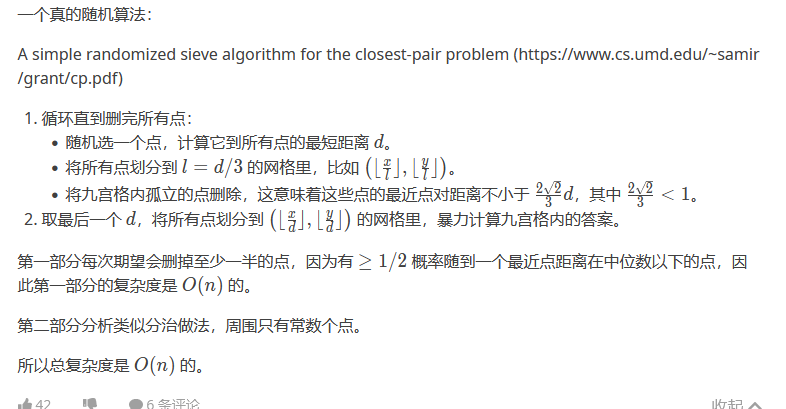
\includegraphics[width=0.8\linewidth]{../src/geometry/最近点对.png}


		\newpage
	
	\begin{multicols}{2}
		\section{杂项}
			\subsection{$O(1)$ 快速乘}
				如果对速度要求很高并且不能用指令集, 可以去看fstqwq的模板.

				\inputminted{cpp}{../src/misc/O(1)快速乘.cpp}
			
			\subsection{Kahan求和算法 (减少浮点数累加的误差)}
				当然一般来说是用不到的, 累加被卡精度了才有必要考虑.
				\inputminted{cpp}{../src/misc/kahan.cpp}
			
			\subsection{Python Decimal}
				\inputminted{python}{../src/misc/decimal.py}
			
			\subsection{$O(n^2)$ 高精度}
				\inputminted{cpp}{../src/misc/高精度.cpp}
			
			\subsection{笛卡尔树}
				\inputminted{cpp}{../src/misc/笛卡尔树.cpp}
			
			\subsection{GarsiaWachs 算法 ($O(n\log n)$ 合并石子)}
				设序列是$\{a_i\}$, 从左往右, 找到一个最小的且满足$a_{k-1} \le a_{k+1}$的$k$, 找到后合并$a_k$和$a_{k-1}$, 再从当前位置开始向左找最大的$j$满足$a_j \ge a_k + a_{k-1}$(当然是指合并前的), 然后把$a_k + a_{k-1}$插到$j$的后面就行. 一直重复, 直到只剩下一堆石子就可以了.

另外在这个过程中, 可以假设$a_{-1}$和$a_n$是正无穷的, 可省略边界的判别. 把$a_0$设为INF, $a_{n+1}$设为INF-1, 可实现剩余一堆石子时自动结束.
			
			\subsection{常用 NTT 素数及原根}
				\begin{tabular}{|c|c|c|c|}
	\hline $p = r \times 2 ^ k + 1$ &  $r$  & $k$  & 最小原根 \\
	\hline $104857601$              &  $25$ & $22$ & $3$ \\
	\hline $167772161$              &  $5$  & $25$ & $3$ \\
     \hline $469762049$      &  $7$   &  $26$  &    $3$ \\
     \hline $\mathbf{985661441}$      & $235$  &  $22$  &    $3$ \\
  \hline $\mathbf{998244353}$    & $119$  &  $23$  &    $3$ \\
  \hline $1004535809$    & $479$  &  $21$  &    $3$ \\
  \hline $1005060097 ^ *$      & $1917$ &  $19$  &  $\emph{5}$ \\
  \hline $\emph{2013265921}$    &  $15$  &  $27$  &  $\emph{31}$ \\
    \hline $2281701377$      &  $17$  &  $27$  &    $3$ \\
 \hline $31525197391593473$  &  $7$   &  $52$  &    $3$ \\
\hline $180143985094819841$  &  $5$   &  $55$  &  $\emph{6}$ \\
\hline $1945555039024054273$ &  $27$  &  $56$  &  $\emph{5}$ \\
\hline $4179340454199820289$ &  $29$  &  $57$  &    $3$ \\
\hline
\end{tabular}

*注: $1005060097$有点危险, 在变化长度大于$524288 = 2 ^ {19}$时不可用.

			\subsection{xorshift}
				\inputminted{cpp}{../src/misc/xorshift.cpp}
			
			\subsection{枚举子集}
				(注意这是$t\ne 0$的写法, 如果可以等于$0$需要在循环里手动\mintinline{cpp}{break})
\begin{minted}{cpp}
for (int t = s; t; (--t) &= s) {
    // do something
}
\end{minted}
				
			\subsection{STL}
				\subsubsection{vector}
	\begin{itemize}
		\item \mintinline{cpp}{vector(int nSize)}: 创建一个vector, 元素个数为nSize
		\item \mintinline{cpp}{vector(int nSize, const T &value)}: 创建一个vector, 元素个数为nSize, 且值均为value
		\item \mintinline{cpp}{vector(begin, end)}: 复制[begin, end)区间内另一个数组的元素到vector中
		\item \mintinline{cpp}{void assign(int n, const T &x)}: 设置向量中前n个元素的值为x
		\item \mintinline{cpp}{void assign(const_iterator first, const_iterator last)}: 向量中[first, last)中元素设置成当前向量元素
		\item \mintinline{cpp}{void emplace_back(Args&&... args)}: 自动构造并push\_back一个元素, 例如对一个存储pair的vector可以 \mintinline{cpp}{v.emplace_back(x, y)}
	\end{itemize}

\subsubsection{list}
	\begin{itemize}
		\item \mintinline{cpp}{assign()} 给list赋值 
		\item \mintinline{cpp}{back()} 返回最后一个元素 
		\item \mintinline{cpp}{begin()} 返回指向第一个元素的迭代器 
		\item \mintinline{cpp}{clear()} 删除所有元素 
		\item \mintinline{cpp}{empty()} 如果list是空的则返回true 
		\item \mintinline{cpp}{end()} 返回末尾的迭代器
		\item \mintinline{cpp}{erase()} 删除一个元素
		\item \mintinline{cpp}{front()} 返回第一个元素
		\item \mintinline{cpp}{insert()} 插入一个元素到list中
		\item \mintinline{cpp}{max_size()} 返回list能容纳的最大元素数量
		\item \mintinline{cpp}{merge()} 合并两个list
		\item \mintinline{cpp}{pop_back()} 删除最后一个元素
		\item \mintinline{cpp}{pop_front()} 删除第一个元素
		\item \mintinline{cpp}{push_back()} 在list的末尾添加一个元素
		\item \mintinline{cpp}{push_front()} 在list的头部添加一个元素
		\item \mintinline{cpp}{rbegin()} 返回指向第一个元素的逆向迭代器
		\item \mintinline{cpp}{remove()} 从list删除元素
		\item \mintinline{cpp}{remove_if()} 按指定条件删除元素
		\item \mintinline{cpp}{rend()} 指向list末尾的逆向迭代器
		\item \mintinline{cpp}{resize()} 改变list的大小
		\item \mintinline{cpp}{reverse()} 把list的元素倒转
		\item \mintinline{cpp}{size()} 返回list中的元素个数
		\item \mintinline{cpp}{sort()} 给list排序
		\item \mintinline{cpp}{splice()} 合并两个list
		\item \mintinline{cpp}{swap()} 交换两个list
		\item \mintinline{cpp}{unique()} 删除list中重复的元
	\end{itemize}

\subsubsection{unordered\_set/map}

\begin{itemize}
	\item \mintinline{cpp}{unordered_map<int, int, hash>}: 自定义哈希函数, 其中hash是一个带重载括号的类.
\end{itemize}

\subsubsection{自定义 Hash}
	\inputminted{cpp}{../src/misc/hash.cpp}

			\subsection{Public Based DataStructure (PB\_DS)}
				\label{pbds}
				\subsubsection{哈希表}

\begin{minted}{cpp}
#include<ext/pb_ds/assoc_container.hpp>
#include<ext/pb_ds/hash_policy.hpp>
using namespace __gnu_pbds;

cc_hash_table<string, int> mp1; // 拉链法
gp_hash_table<string, int> mp2; // 查探法(快一些)
\end{minted}

\subsubsection{堆}

默认也是大根堆, 和\mintinline{cpp}{std::priority_queue}保持一致.

\begin{minted}{cpp}
#include<ext/pb_ds/priority_queue.hpp>
using namespace __gnu_pbds;

__gnu_pbds::priority_queue<int> q;
__gnu_pbds::priority_queue<int, greater<int>, pairing_heap_tag> pq;
\end{minted}

效率参考:

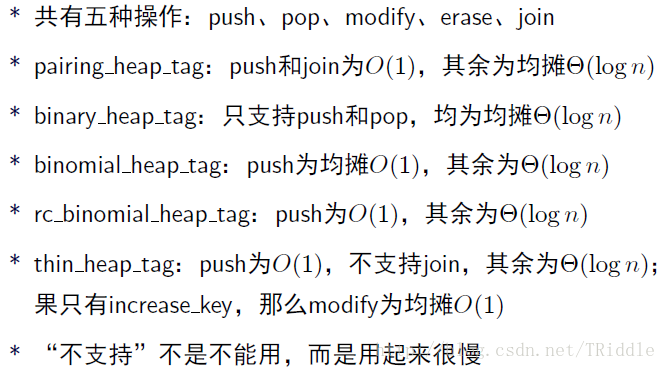
\includegraphics[scale = 0.385]{../src/misc/pbds_heap.png}

常用操作:

\begin{itemize}

	\item \mintinline{cpp}{push()}: 向堆中压入一个元素, 返回迭代器
	\item \mintinline{cpp}{pop()}: 将堆顶元素弹出
	\item \mintinline{cpp}{top()}: 返回堆顶元素
	\item \mintinline{cpp}{size()}: 返回元素个数
	\item \mintinline{cpp}{empty()}: 返回是否非空
	\item \mintinline{cpp}{modify(point_iterator, const key)}: 把迭代器位置的 \mintinline{cpp}{key} 修改为传入的 \mintinline{cpp}{key}
	\item \mintinline{cpp}{erase(point_iterator)}: 把迭代器位置的键值从堆中删除
	\item \mintinline{cpp}{join(__gnu_pbds::priority_queue &other)}: 把 \mintinline{cpp}{other} 合并到 \mintinline{cpp}{*this}, 并把 \mintinline{cpp}{other} 清空
\end{itemize}

\subsubsection{平衡树}

\begin{minted}{cpp}
#include <ext/pb_ds/tree_policy.hpp>
#include <ext/pb_ds/assoc_container.hpp>
using namespace __gnu_pbds;

tree<int, null_type, less<int>, rb_tree_tag, tree_order_statistics_node_update> t;

// rb_tree_tag 红黑树(还有splay_tree_tag和ov_tree_tag, 后者不知道是什么)
\end{minted}

注意第五个参数要填\mintinline{cpp}{tree_order_statistics_node_update}才能使用排名操作.

\begin{itemize}
	\item \mintinline{cpp}{insert(x)}: 向树中插入一个元素x, 返回\mintinline{cpp}{pair<point_iterator, bool>}
	\item \mintinline{cpp}{erase(x)}: 从树中删除一个元素/迭代器x, 返回一个 \mintinline{cpp}{bool} 表明是否删除成功
	\item \mintinline{cpp}{order_of_key(x)}: 返回x的排名, 0-based
	\item \mintinline{cpp}{find_by_order(x)}: 返回排名(0-based)所对应元素的迭代器
	\item \mintinline{cpp}{lower_bound(x) / upper_bound(x)}: 返回第一个$\ge$或者>x的元素的迭代器
	\item \mintinline{cpp}{join(x)}: 将x树并入当前树, 前提是两棵树的类型一样, 并且二者值域不能重叠, x树会被删除
	\item \mintinline{cpp}{split(x,b)}: 分裂成两部分, 小于等于x的属于当前树, 其余的属于b树
	\item \mintinline{cpp}{empty()}: 返回是否为空
	\item \mintinline{cpp}{size()}: 返回大小
\end{itemize}

(注意平衡树不支持多重值, 如果需要多重值, 可以再开一个\mintinline{cpp}{unordered_map}来记录值出现的次数, 将\mintinline{cpp}{x<<32}后加上出现的次数后插入. 注意此时应该为long long类型.)

			\subsection{rope}
				\inputminted{cpp}{../src/misc/rope.cpp}
			
			\subsection{其他 C++ 相关}
				\subsubsection{<cmath>}

\begin{itemize}
	\item \mintinline{cpp}{std::log1p(x)}: (注意是数字1)返回$\ln(1 + x)$的值, $x$非常接近$0$时比直接exp精确得多.
	\item \mintinline{cpp}{std::hypot(x, y[, z])}: 返回平方和的平方根, 或者说到原点的欧几里德距离.
\end{itemize}

\subsubsection{<algorithm>}

\begin{itemize}
	\item \mintinline{cpp}{std::all_of(begin, end, f)}: 检查范围内元素调用函数f后是否全返回真. 类似地还有\mintinline{cpp}{std::any_of}和\mintinline{cpp}{std::none_of}.
	\item \mintinline{cpp}{std::for_each(begin, end, f)}: 对范围内所有元素调用一次f. 如果传入的是引用, 也可以用f修改. (例如\mintinline{cpp}{for_each(a, a + n, [](int &x){cout << ++x << "\n";})})
	\item \mintinline{cpp}{std::for_each_n(begin, n, f)}: 同上, 只不过范围改成了从begin开始的n个元素.
	\item \mintinline{cpp}{std::copy(), std::copy_n()}: 用法谁都会, 但标准里说如果元素是可平凡复制的(比如int), 那么它会避免批量赋值, 并且调用\mintinline{cpp}{std::memmove()}之类的快速复制函数. (一句话总结: 它跑得快)
	\item \mintinline{cpp}{std::rotate(begin, mid, end)}: 循环移动, 移动后mid位置的元素会跑到first位置. C++11起会返回begin位置的元素移动后的位置.
	\item \mintinline{cpp}{std::unique(begin, end)}: 去重, 返回去重后的end.
	\item \mintinline{cpp}{std::partition(begin, end, f)}: 把f为true的放在前面, false的放在后面, 返回值是第二部分的开头, \textbf{不保持相对顺序}. 如果要保留相对顺序可以用\mintinline{cpp}{std::stable_partition()}, 比如写整体二分.
	\item \mintinline{cpp}{std::partition_copy(begin, end, begin_t, begin_f, f)}: 不修改原数组, 把true的扔到begin\_t, false的扔到begin\_f. 返回值是两部分结尾的迭代器的pair.
	\item \mintinline{cpp}{std::equal_range(begin, end, x)}: 在已经排好序的数组里找到等于x的范围.
	\item \mintinline{cpp}{std::minmax(a, b)}: 返回\mintinline{cpp}{pair(min(a, b), max(a, b))}. 比如\mintinline{cpp}{tie(l, r) = minmax(l, r)}.
\end{itemize}

\subsubsection{std::tuple}

\begin{itemize}
	\item \mintinline{cpp}{std::make_tuple(...)}: 返回构造好的tuple
	\item \mintinline{cpp}{std::get<i>(tup)}: 返回tuple的第i项
	\item \mintinline{cpp}{std::tuple_cat(...)}: 传入几个tuple, 返回按顺序连起来的tuple
	\item \mintinline{cpp}{std::tie(x, y, z, ...)}: 把传入的变量的左值引用绑起来作为tuple返回, 例如可以\mintinline{cpp}{std::tie(x, y, z) = std::make_tuple(a, b, c)}.
\end{itemize}

\subsubsection{<complex>}

\begin{itemize}
	\item \mintinline{cpp}{complex<double> imaginary = 1i, x = 2 + 3i}: 可以这样直接构造复数.
	\item \mintinline{cpp}{real/imag(x)}: 返回实部/虚部.
	\item \mintinline{cpp}{conj(x)}: 返回共轭复数.
	\item \mintinline{cpp}{arg(x)}: 返回辐角.
	\item \mintinline{cpp}{norm(x)}: 返回模的平方. (直接求模用\mintinline{cpp}{abs(x)}.)
	\item \mintinline{cpp}{polar(len, theta)}: 用绝对值和辐角构造复数.
\end{itemize}
			
			\subsection{一些游戏}
				\subsubsection{德州扑克}
					一般来说德扑里 Ace 都是最大的,所以把 Ace 的点数规定为 $14$ 会好写许多。

附一个高低奥马哈的参考代码,除了有四张底牌和需要比低之外和德扑区别不大。

\inputminted{cpp}{../src/misc/高低奥马哈.cpp}


				\subsubsection{炉石传说}
					两个随从$(a_i, h_i)$和$(a_j, h_j)$皇城PK, 最后只有$a_i\times h_i$较大的一方才有可能活下来, 当然也有可能一起死.

			\subsection{OEIS}
				\label{oeis}
				如果没有特殊说明,那么以下数列都从第 $0$ 项开始,除非没有定义也没有好的办法解释第 $0$ 项的意义。

\subsubsection{计数相关}

\begin{enumerate}

\item \textbf{卡特兰数 A000108)}

1, 1, 2, 5, 14, 42, 132, 429, 1430, 4862, 16796, 58786, 208012, 742900, 2674440, 9694845, 35357670, \dots

性质见 \detailedref{catalan}。 

\item \textbf{(大)施罗德数 A006318}

1, 2, 6, 22, 90, 394, 1806, 8558, 41586, 206098, 1037718, 5293446, 27297738, 142078746, 745387038, \dots \;(0-based)

性质同样见 \detailedref{catalan}。

\item \textbf{小施罗德数 A001003}

1, 1, 3, 11, 45, 197, 903, 4279, 20793, 103049, 518859, 2646723, 13648869, 71039373, 372693519, \dots \;(0-based)

性质位置同上。

小施罗德数除了第 $0$ 项以外都是施罗德数的一半。

\item \textbf{默慈金数(Motzkin numbers) A001006}

1, 1, 2, 4, 9, 21, 51, 127, 323, 835, 2188, 5798, 15511, 41835, 113634, 310572, 853467, 2356779, \dots \;(0-based)

性质位置同上。

\item \textbf{将点按顺序排成一圈后不自交的树的个数 A001764}

1, 1, 3, 12, 55, 273, 1428, 7752, 43263, 246675, 1430715, 8414640, 50067108, 300830572, 1822766520, \dots \;(0-based)

$ a_n = \frac {{3n \choose n}} {2n + 1} $

也就是说,在圆上按顺序排列的 $n$ 个点之间连 $n - 1$ 条不相交(除端点外)的弦,组成一棵树的方案数。

也等于每次只能向右或向上,并且不能高于 $y = 2x$ 这条直线,从 $(0, 0)$ 走到 $(n, 2n)$ 的方案数。

\paragraph{扩展} 如果改成不能高于 $y = kx$ 这条直线,走到$(n, kn)$ 的方案数,那么答案就是$ \frac {{(k + 1)n \choose n}} {kn + 1} $。

\item \textbf{$n$ 个点的圆上画不相交的弦的方案数 A054726}

1, 1, 2, 8, 48, 352, 2880, 25216, 231168, 2190848, 21292032, 211044352, 2125246464, 21681954816, \dots \;(0-based)

$ a_n = 2^n s_{n - 2} \; (n > 2) $,其中 $s_n$ 是上面的小施罗德数。

和上面的区别在于,这里可以不连满 $n-1$ 条边。另外默慈金数画的弦不能共享端点,但是这里可以。

\item \textbf{Wedderburn-Etherington numbers A001190}

0, 1, 1, 1, 2, 3, 6, 11, 23, 46, 98, 207, 451, 983, 2179, 4850, 10905, 24631, 56011, 127912, 293547, \dots \;(0-based)

每个结点都有 $0$ 或者 $2$ 个儿子,且总共有 $n$ 个叶子结点的二叉树方案数。(\textbf{无标号})

同时也是 $n-1$ 个结点的 \textbf{无标号}\ 二叉树个数。

$ A(x) = x + \frac {A(x) ^ 2 + A(x ^ 2)} 2 = 1 - \sqrt{1 - 2x - A(x ^ 2)} $
	
\item \textbf{分拆数 A000041}

1, 1, 2, 3, 5, 7, 11, 15, 22, 30, 42, 56, 77, 101, 135, 176, 231, 297, 385, 490, 627, 792, 1002, \dots \;(0-based)

性质见 \detailedref{partition}。

\item \textbf{贝尔数 A000110}

1, 1, 2, 5, 15, 52, 203, 877, 4140, 21147, 115975, 678570, 4213597, 27644437, 190899322, 1382958545, \dots \;(0-based)

性质见 \detailedref{BellNumber}。

\item \textbf{错位排列数 A0000166}

1, 0, 1, 2, 9, 44, 265, 1854, 14833, 133496, 1334961, 14684570, 176214841, 2290792932, 32071101049, \dots \;(0-based)

\item \textbf{交替阶乘 A005165}

0, 1, 1, 5, 19, 101, 619, 4421, 35899, 326981, 3301819, 36614981, 442386619, 5784634181, 81393657019, \dots \; (0-based)

$ \begin{aligned} n! - (n - 1)! + (n - 2)! - \dots 1! = \sum_{i = 0} ^ {n - 1} (-1)^i (n - i)! \end{aligned} $

$ a_0 = 0,\; a_n = n! - a_{n - 1} $

\end{enumerate}

\subsubsection{线性递推数列}

\begin{enumerate}

\item \textbf{Lucas 数 A000032}

2, 1, 3, 4, 7, 11, 18, 29, 47, 76, 123, 199, 322, 521, 843, 1364, 2207, 3571, 5778, 9349, 15127, \dots

\item \textbf{斐波那契数 A000045}

0, 1, 1, 2, 3, 5, 8, 13, 21, 34, 55, 89, 144, 233, 377, 610, 987, 1597, 2584, 4181, 6765, 10946, \dots

\item \textbf{泰波那契数(Tribonacci) A000071}

0, 0, 1, 1, 2, 4, 7, 13, 24, 44, 81, 149, 274, 504, 927, 1705, 3136, 5768, 10609, 19513, 35890, \dots

$ a_0 = a_1 = 0,\; a_2 = 1,\; a_n = a_{n - 1} + a_{n - 2} + a_{n - 3} $

\item \textbf{Pell 数 A0000129}

0, 1, 2, 5, 12, 29, 70, 169, 408, 985, 2378, 5741, 13860, 33461, 80782, 195025, 470832, 1136689, \dots

$ a_0 = 0,\; a_1 = 1,\; a_n = 2a_{n - 1} + a_{n - 2} $

\item \textbf{Padovan 数 A0000931}

1, 0, 0, 1, 0, 1, 1, 1, 2, 2, 3, 4, 5, 7, 9, 12, 16, 21, 28, 37, 49, 65, 86, 114, 151, 200, 265, 351, 465, 616, 816, 1081, 1432, 1897, 2513, 3329, 4410, 5842, 7739, 10252, 13581, 17991, 23833, 31572, \dots

$a_0 = 1,\; a_1 = a_2 = 0,\; a_n = a_{n - 2} + a_{n - 3}$

\item \textbf{Jacobsthal numbers A001045}

0, 1, 1, 3, 5, 11, 21, 43, 85, 171, 341, 683, 1365, 2731, 5461, 10923, 21845, 43691, 87381, 174763, \dots

$ a_0 = 0,\; a_1 = 1.\; a_n = a_{n - 1} + 2a_{n - 2} $

同时也是最接近 $\frac {2 ^ n} 3$ 的整数。

\item \textbf{佩林数 A001608}

3, 0, 2, 3, 2, 5, 5, 7, 10, 12, 17, 22, 29, 39, 51, 68, 90, 119, 158, 209, 277, 367, 486, 644, 853, \dots

$ a_0 = 3,\; a_1 = 0,\; a_2 = 2,\; a_n = a_{n - 2} + a_{n - 3} $

\end{enumerate}

\subsubsection{数论相关}

\begin{enumerate}

\item \textbf{Carmichael 数/伪质数 A002997}

561, 1105, 1729, 2465, 2821, 6601, 8911, 10585, 15841, 29341, 41041, 46657, 52633, 62745, 63973, 75361, 101101, 115921, 126217, 162401, 172081, 188461, 252601, 278545, 294409, 314821, 334153, 340561, 399001, 410041, 449065, 488881, 512461, \dots

满足 $\forall$ 与 $n$ 互质的 $a$,都有 $a ^ {n - 1} \equiv 1 \pmod n$ 的所有 \textbf{合数}\ $n$ 被称为 Carmichael 数。

Carmichael 数在 $10^8$ 以内只有255个。

\item \textbf{反质数 A002182}

1, 2, 4, 6, 12, 24, 36, 48, 60, 120, 180, 240, 360, 720, 840, 1260, 1680, 2520, 5040, 7560, 10080, 15120, 20160, 25200, 27720, 45360, 50400, 55440, 83160, 110880, 166320, 221760, 277200, 332640, 498960, 554400, 665280, 720720, 1081080, 1441440, 2162160, \dots

比所有更小的数的约数数量都更多的数。

\item \textbf{前 $n$ 个质数的乘积 A002110}

1, 2, 6, 30, 210, 2310, 30030, 510510, 9699690, 223092870, 6469693230, 200560490130, 7420738134810, \dots

\item \textbf{梅森质数 A000668}

3, 7, 31, 127, 8191, 131071, 524287, 2147483647, 2305843009213693951, 618970019642690137449562111, 162259276829213363391578010288127,\\170141183460469231731687303715884105727

$p$ 是质数,同时 $2^p - 1$ 也是质数。

\end{enumerate}

\subsubsection{其他}

\begin{enumerate}

\item \textbf{伯努利数 A027641}

参见 \detailedref{BernoulliNumber}。

(伯努利数并不是整数。)

\item \textbf{四个柱子的汉诺塔 A007664}

0, 1, 3, 5, 9, 13, 17, 25, 33, 41, 49, 65, 81, 97, 113, 129, 161, 193, 225, 257, 289, 321, 385, 449, \dots

差分之后可以发现其实就是 $1$ 次 $+1$,$2$ 次 $+2$,$3$ 次 $+4$,$4$ 次 $+8$ \dots 的规律。

\item \textbf{乌拉姆数(Ulam numbers) A002858}

1, 2, 3, 4, 6, 8, 11, 13, 16, 18, 26, 28, 36, 38, 47, 48, 53, 57, 62, 69, 72, 77, 82, 87, 97, 99, 102, 106, 114, 126, 131, 138, 145, 148, 155, 175, 177, 180, 182, 189, 197, 206, 209, 219, 221, 236, 238, 241, 243, 253, 258, 260, 273, 282, 309, 316, 319, 324, 339,\dots

$ a_1 = 1,\; a_2 = 2 $,$a_n$ 表示在所有 $>a_{n-1}$ 的数中,最小的、能被表示成前面的两个 \textbf{不同}\ 的元素的和的数。

\end{enumerate}

			
			\subsection{编译选项}
				\begin{itemize}
	\item \mintinline{cpp}{-O2 -g -std=c++17}: 狗都知道
	\item \mintinline{cpp}{-Wall -Wextra -Wshadow -Wconversion}: 更多警告
		\subitem --\; \mintinline{cpp}{-Werror}: 强制将所有Warning变成Error
	\item \mintinline{cpp}{-fsanitize=(address/undefined/ftrapv)}: 检查数组越界/有符号整数溢出(算ub)
		\subitem --\;调试神器, 在遇到错误时会输出信息.
		\subitem --\;注意无符号类型溢出不算ub.
	\item \mintinline{cpp}{-fno-ms-extensions}: 关闭一些和msvc保持一致的特性, 例如, 不标返回值类型的函数会报CE而不是默认为\mintinline{cpp}{int}.
		\subitem --\;但是不写return的话它还是管不了.
	\item \mintinline{cpp}{#define debug(x) cout << #x << " = " << x << endl}
\end{itemize}
				
			% \subsection{注意事项}

			% 	\subsubsection{常见下毒手法}
			% 		\noindent
\begin{itemize}
    \item 高精度高低位搞反了吗
    \item 线性筛抄对了吗
    \item 快速乘抄对了吗
    \item \mintinline{cpp}{i <= n, j <= m}
    \item sort比较函数是不是比了个寂寞
    \item 该取模的地方都取模了吗
    \item 边界情况(+1-1之类的)有没有想清楚
    \item \bfseries{特判是否有必要, 确定写对了吗}
\end{itemize}

			% 	\subsubsection{场外相关}
			% 		\noindent
\begin{itemize}
    \item 安顿好之后查一下附近的咖啡店,打印店,便利店之类的位置,以备不时之需
    \item 热身赛记得检查一下编译注意事项中的代码能否过编译,还有熟悉比赛场地,清楚洗手间在哪儿,测试打印机(如果可以)
    \item 比赛前至少要翻一遍板子,尤其要看原理与例题
    \item 比赛前一两天不要摸鱼,要早睡,有条件最好洗个澡;比赛当天不要起太晚,维持好的状态
    \item 赛前记得买咖啡,最好直接安排三人份,记得要咖啡因比较足的;如果主办方允许,就带些巧克力之类的高热量零食
    \item 入场之后记得检查机器,尤其要逐个检查键盘按键有没有坏的;如果可以的话,调一下gedit设置
    \item 开赛之前调整好心态,比赛而已,不必心急.
\end{itemize}

			% 	\subsubsection{做题策略与心态调节}
			% 		\noindent
\begin{itemize}
	\item 拿到题后立刻按照商量好的顺序读题,前半小时最好跳过题意太复杂的题(除非被过穿了)
	
	\item 签到题写完不要激动,稍微检查一下最可能的下毒点再交,避免无谓的罚时
		\begin{itemize}
			\item 一两行的那种傻逼题就算了
		\end{itemize}
		
	\item 读完题及时输出题意,一方面避免重复读题,一方面也可以让队友有一个初步印象,方便之后决定开题顺序
	
	\item 如果不能确定题意就不要贸然输出甚至上机, 尤其是签到题, 因为样例一般都很弱
	
	\item —个题如果卡了很久又有其他题可以写,那不妨先放掉写更容易的题,不要在一棵树上吊死
		\begin{itemize}
			\item 不要被—两道题搞得心态爆炸,一方面急也没有意义,一方面你很可能真的离AC就差一步
		\end{itemize}
		
	\item 榜是不会骗人的,一个题如果被不少人过了就说明这个题很可能并没有那么难;如果不是有十足的把握就不要轻易开没什么人交的题;另外不要忘记最后一小时会封榜
	
	\item 想不出题/找不出毒自然容易犯困,一定不要放任自己昏昏欲睡,最好去洗手间冷静一下,没有条件就站起来踱步
	
	\item 思考的时候不要挂机,一定要在草稿纸上画一画,最好说出声来最不容易断掉思路
	
	\item 出完算法一定要check一下样例和一些trivial的情况,不然容易写了半天发现写了个假算法
	
	\item 上机前有时间就提前给需要思考怎么写的地方打草稿,不要浪费机时
	
	\item 查毒时如果最难的地方反复check也没有问题,就从头到脚仔仔细细查一遍,不要放过任何细节,即使是并查集和sort这种东西也不能想当然
	
	\item 后半场如果时间不充裕就不要冒险开难题,除非真的无事可做
		\begin{itemize}
			\item 如果是没写过的东西也不要轻举妄动,在有其他好写的题的时候就等一会再说
		\end{itemize}
		
	\item 大多数时候都要听队长安排,虽然不一定最正确但可以保持组织性
	
	\item 最好注意一下影响,就算忍不住嘴臭也不要太大声
	
	\item 任何时候都不要着急,着急不能解决问题,不要当喆国王
	
	\item 输了游戏,还有人生;赢了游戏,还有人生.
\end{itemize}
			
			\subsection{附录: VScode 相关}
				\subsubsection{插件}

\begin{itemize}
	\item Chinese (Simplified) (简体中文语言包)
	\item C/C++
	\item C++ Intellisense (前提是让用)
	\item Better C++ Syntax
	\item Python
	\item Pylance (前提是让用)
	\item Rainbow Brackets (前提是让用)
\end{itemize}

\subsubsection{设置选项}

\begin{itemize}
	\item Editor: Insert Spaces (取消勾选, 改为tab缩进)
	\item Editor: Line Warp (开启折行)
	\item 改配色, ``深色+: 默认深色''
	\item 自动保存(F1 $\rightarrow$ ``auto'')
	\item Terminal $\to$ Integrated: Cursor Style (修改终端光标形状)
	\item Terminal $\to$ Integrated: Cursor Blinking (终端光标闪烁)
	\item 字体改为Cascadia Code/Mono SemiLight (Windows可用)
\end{itemize}

\subsubsection{快捷键}

\begin{itemize}
	\item F1 / Ctrl+Shift+P: 万能键, 打开命令面板
	\item F8: 下一个Error \quad Shift+F8: 上一个Error
	\item Ctrl+$\backslash$: 水平分栏, 最多3栏
	\item Ctrl+1/2/3: 切到对应栏
	\item Ctrl+[/]: 当前行向左/右缩进
	\item Alt+F12: 查看定义的缩略图(显示小窗, 不跳过去)
	\item Ctrl+H: 查找替换
	\item Ctrl+D: 下一个匹配的也被选中(用于配合Ctrl+F)
	\item Ctrl+U: 回退上一个光标操作(防止光标飞了找不回去)
	\item Ctrl+/: 切换行注释
	\item Ctrl+\text{`}(键盘左上角的倒引号): 显示终端
\end{itemize}
			
			\newpage
			\subsection{附录: 骂人的艺术—梁实秋}
				
\hspace{2em}古今中外没有一个不骂人的人。骂人就是有道德观念的意思,因为在骂人的时候,至少在骂人者自己总觉得那人有该骂的地方。何者该骂,何者不该骂,这个抉择的标准,是极道德的。所以根本不骂人,大可不必。骂人是一种发泄感情的方法,尤其是那一种怨怒的感情。想骂人的时候而不骂,时常在身体上弄出毛病,所以想骂人时,骂骂何妨?

\hspace{2em}但是,骂人是一种高深的学问,不是人人都可以随便试的。有因为骂人挨嘴巴的,有因为骂人吃官司的,有因为骂人反被人骂的,这都是不会骂人的原故。今以研究所得,公诸同好,或可为骂人时之一助乎?

\begin{enumerate}

\item 知己知彼

\hspace{1.8em}骂人是和动手打架一样的,你如其敢打人一拳,你先要自己忖度下,你吃得起别人的一拳否。这叫做知己知彼。骂人也是一样。譬如你骂他是“屈死”,你先要反省,自己和“屈死”有无分别。你骂别人荒唐,你自己想想曾否吃喝嫖赌。否则别人回敬你一二句,你就受不了。所以别人有着某种短处,而足下也正有同病,那么你在骂他的时候只得割爱。

\item 无骂不如己者

\hspace{1.8em}要骂人须要挑比你大一点的人物,比你漂亮一点的或者比你坏得万倍而比你得势的人物,总之,你要骂人,那人无论在好的一方面或坏的一方面都要能胜过你,你才不吃亏。你骂大人物,就怕他不理你,他一回骂,你就算骂着了。因为身份相同的人才肯对骂。在坏的一方面胜过你的,你骂他就如教训一般,他既便回骂,一般人仍不会理会他的。假如你骂一个无关痛痒的人,你越骂他他越得意,时常可以把一个无名小卒骂出名了,你看冤与不冤?

\item 适可而止

\hspace{1.8em}骂大人物骂到他回骂的时候,便不可再骂;再骂则一般人对你必无同情,以为你是无理取闹。骂小人物骂到他不能回骂的时候,便不可再骂;再骂下去则一般人对你也必无同情,以为你是欺负弱者。

\item 旁敲侧击

\hspace{1.8em}他偷东西,你骂他是贼;他抢东西,你骂他是盗,这是笨伯。骂人必须先明虚实掩映之法,须要烘托旁衬,旁敲侧击,于要紧处只一语便得,所谓杀人于咽喉处着刀。越要骂他你越要原谅他,即便说些恭维话亦不为过,这样的骂法才能显得你所骂的句句是真实确凿,让旁人看起来也可见得你的度量。

\item 态度镇定

\hspace{1.8em}骂人最忌浮躁。一语不合,面红筋跳,暴躁如雷,此灌夫骂座,泼妇骂街之术,不足以言骂人。善骂者必须态度镇静,行若无事。普通一般骂人,谁的声音高便算谁占理,谁的来势猛便算谁骂赢,惟真善骂人者,乃能避其锋而击其懈。你等他骂得疲倦的时候,你只消轻轻的回敬他一句,让他再狂吼一阵。在他暴躁不堪的时候,你不妨对他冷笑几声,包管你不费力气,把他气得死去活来,骂得他针针见血。

\item 出言典雅

\hspace{1.8em}骂人要骂得微妙含蓄,你骂他一句要使他不甚觉得是骂,等到想过一遍才慢慢觉悟这句话不是好话,让他笑着的面孔由白而红,由红而紫,由紫而灰,这才是骂人的上乘。欲达到此种目的,深刻之用意固不可少,而典雅之言词则尤为重要。言词典雅可使听者不致刺耳。如要骂人骂得典雅,则首先要在骂时万万别提起女人身上的某一部分,万万不要涉及生理学范围。骂人一骂到生理学范围以内,底下再有什么话都不好说了。譬如你骂某甲,千万别提起他的令堂令妹。因为那样一来,便无是非可言,并且你自己也不免有令堂令妹,他若回敬起来,岂非势均力敌,半斤八两?再者骂人的时候,最好不要加人以种种难堪的名词,称呼起来总要客气,即使他是极卑鄙的小人,你也不妨称他先生,越客气,越骂得有力量。骂得时节最好引用他自己的词句,这不但可以使他难堪,还可以减轻他对你骂的力量。俗话少用,因为俗话一览无遗,不若典雅古文曲折含蓄。

\item 以退为进

\hspace{1.8em}两人对骂,而自己亦有理屈之处,则处于开骂伊始,特宜注意,最好是毅然将自己理屈之处完全承认下来,即使道歉认错均不妨事。先把自己理屈之处轻轻遮掩过去,然后你再重整旗鼓,着着逼人,方可无后顾之忧。即使自己没有理屈的地方,也绝不可自行夸张,务必要谦逊不遑,把自己的位置降到一个不可再降的位置,然后骂起人来,自有一种公正光明的态度。否则你骂他一两句,他便以你个人的事反唇相讥,一场对骂,会变成两人私下口角,是非曲直,无从判断。所以骂人者自己要低声下气,此所谓以退为进。

\item 预设埋伏

\hspace{1.8em}你把这句话骂过去,你便要想想看,他将用什么话骂回来。有眼光的骂人者,便处处留神,或是先将他要骂你的话替他说出来,或是预先安设埋伏,令他骂回来的话失去效力。他骂你的话,你替他说出来,这便等于缴了他的械一般。预设埋伏,便是在要攻击你的地方,你先轻轻的安下话根,然后他骂过来就等于枪弹打在沙包上,不能中伤。

\item 小题大做

\hspace{1.8em}如对方有该骂之处,而题目身小,不值一骂,或你所知不多,不足一骂,那时节你便可用小题大做的方法,来扩大题目。先用诚恳而怀疑的态度引申对方的意思,由不紧要之点引到大题目上去,处处用严谨的逻辑逼他说出不逻辑的话来,或是逼他说出合于逻辑但不合乎理的话来,然后你再大举骂他,骂到体无完肤为止,而原来惹动你的小题目,轻轻一提便了。

\item 远交近攻

\hspace{1.8em}一个时候,只能骂一个人,或一种人,或一派人。决不宜多树敌。所以骂人的时候,万勿连累旁人,即使必须牵涉多人,你也要表示好意,否则回骂之声纷至沓来,使你无从应付。

\end{enumerate}

\hspace{2em}骂人的艺术,一时所能想起来的有上面十条,信手拈来,并无条理。我做此文的用意,是助人骂人。同时也是想把骂人的技术揭破一点,供爱骂人者参考。挨骂的人看看,骂人的心理原来是这样的,也算是揭破一张黑幕给你瞧瞧!

			
			\subsection{附录: Cheat Sheet}
				见后面几页.

	\end{multicols}

	\includepdf[pages = 1-10]{../src/misc/Cheat.pdf}

	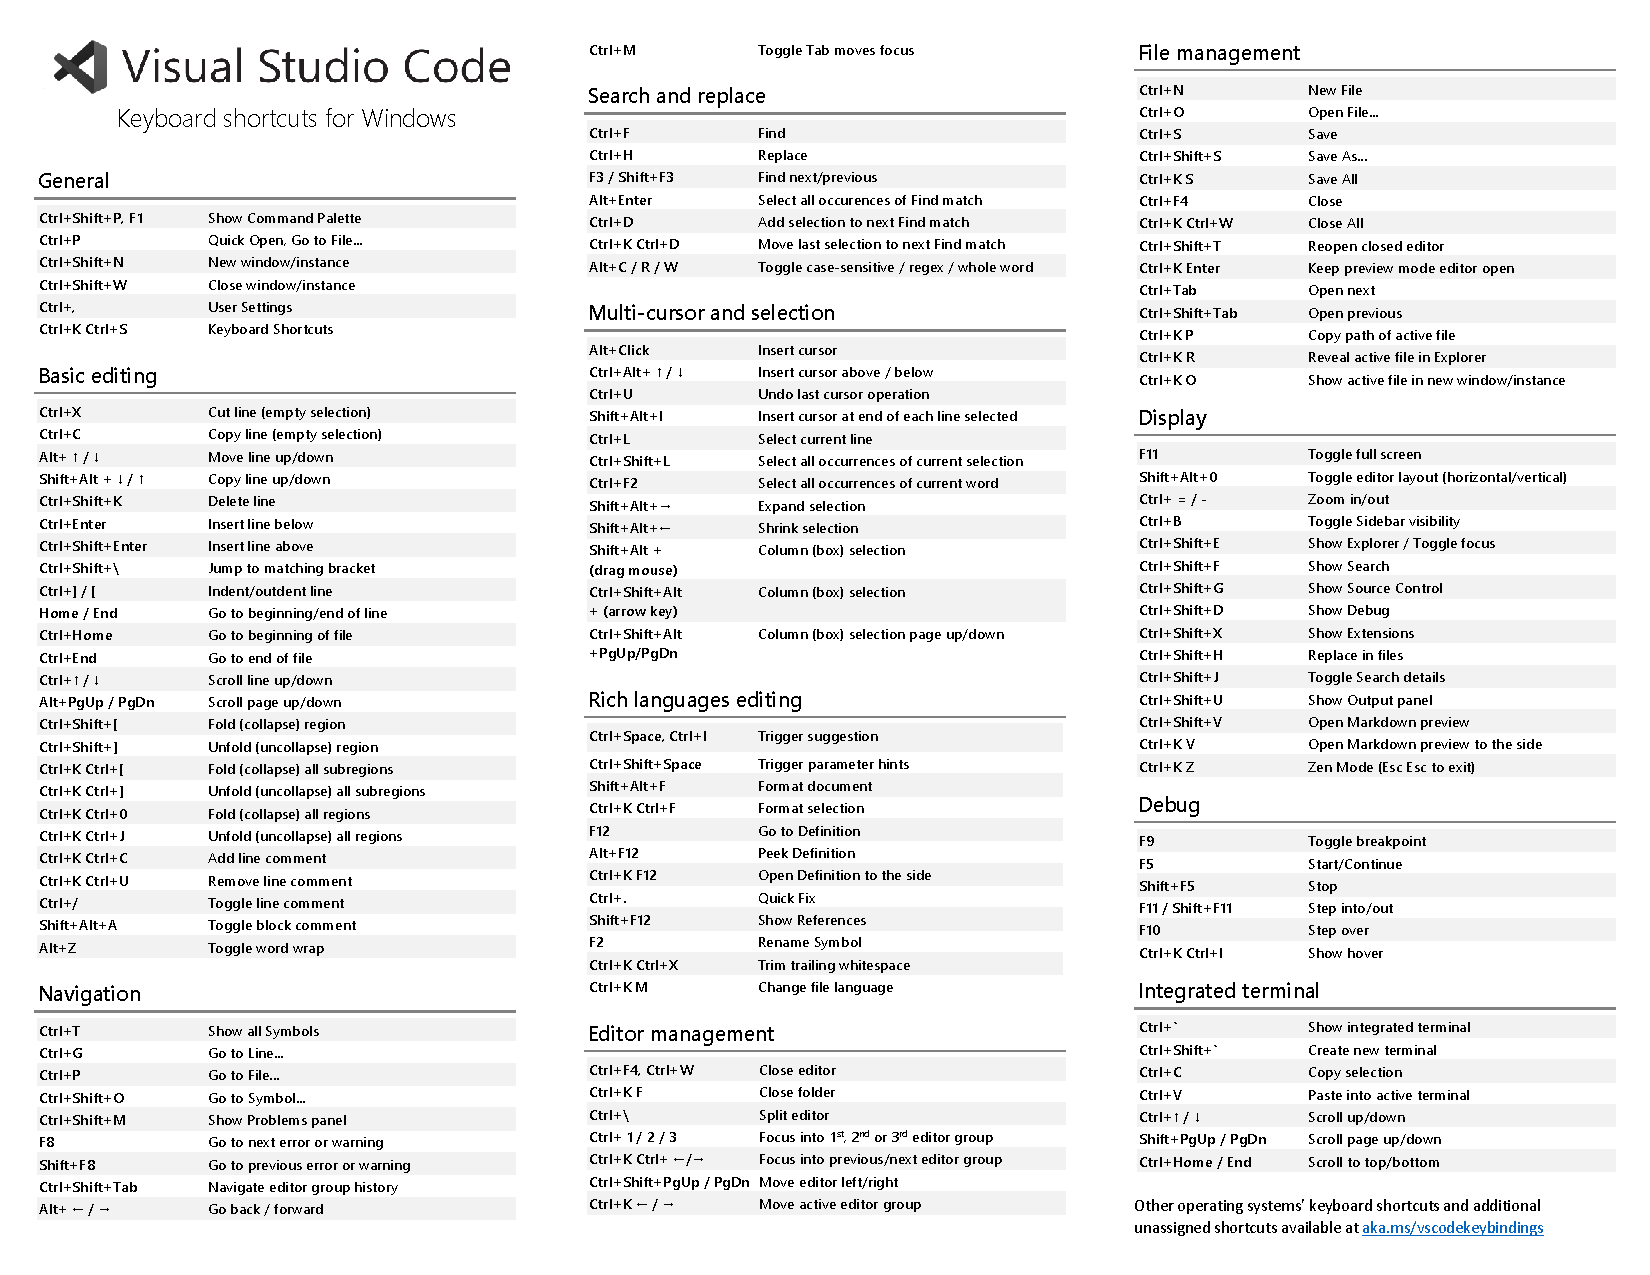
\includepdf[angle=90]{../src/misc/keyboard-shortcuts-windows.pdf}

	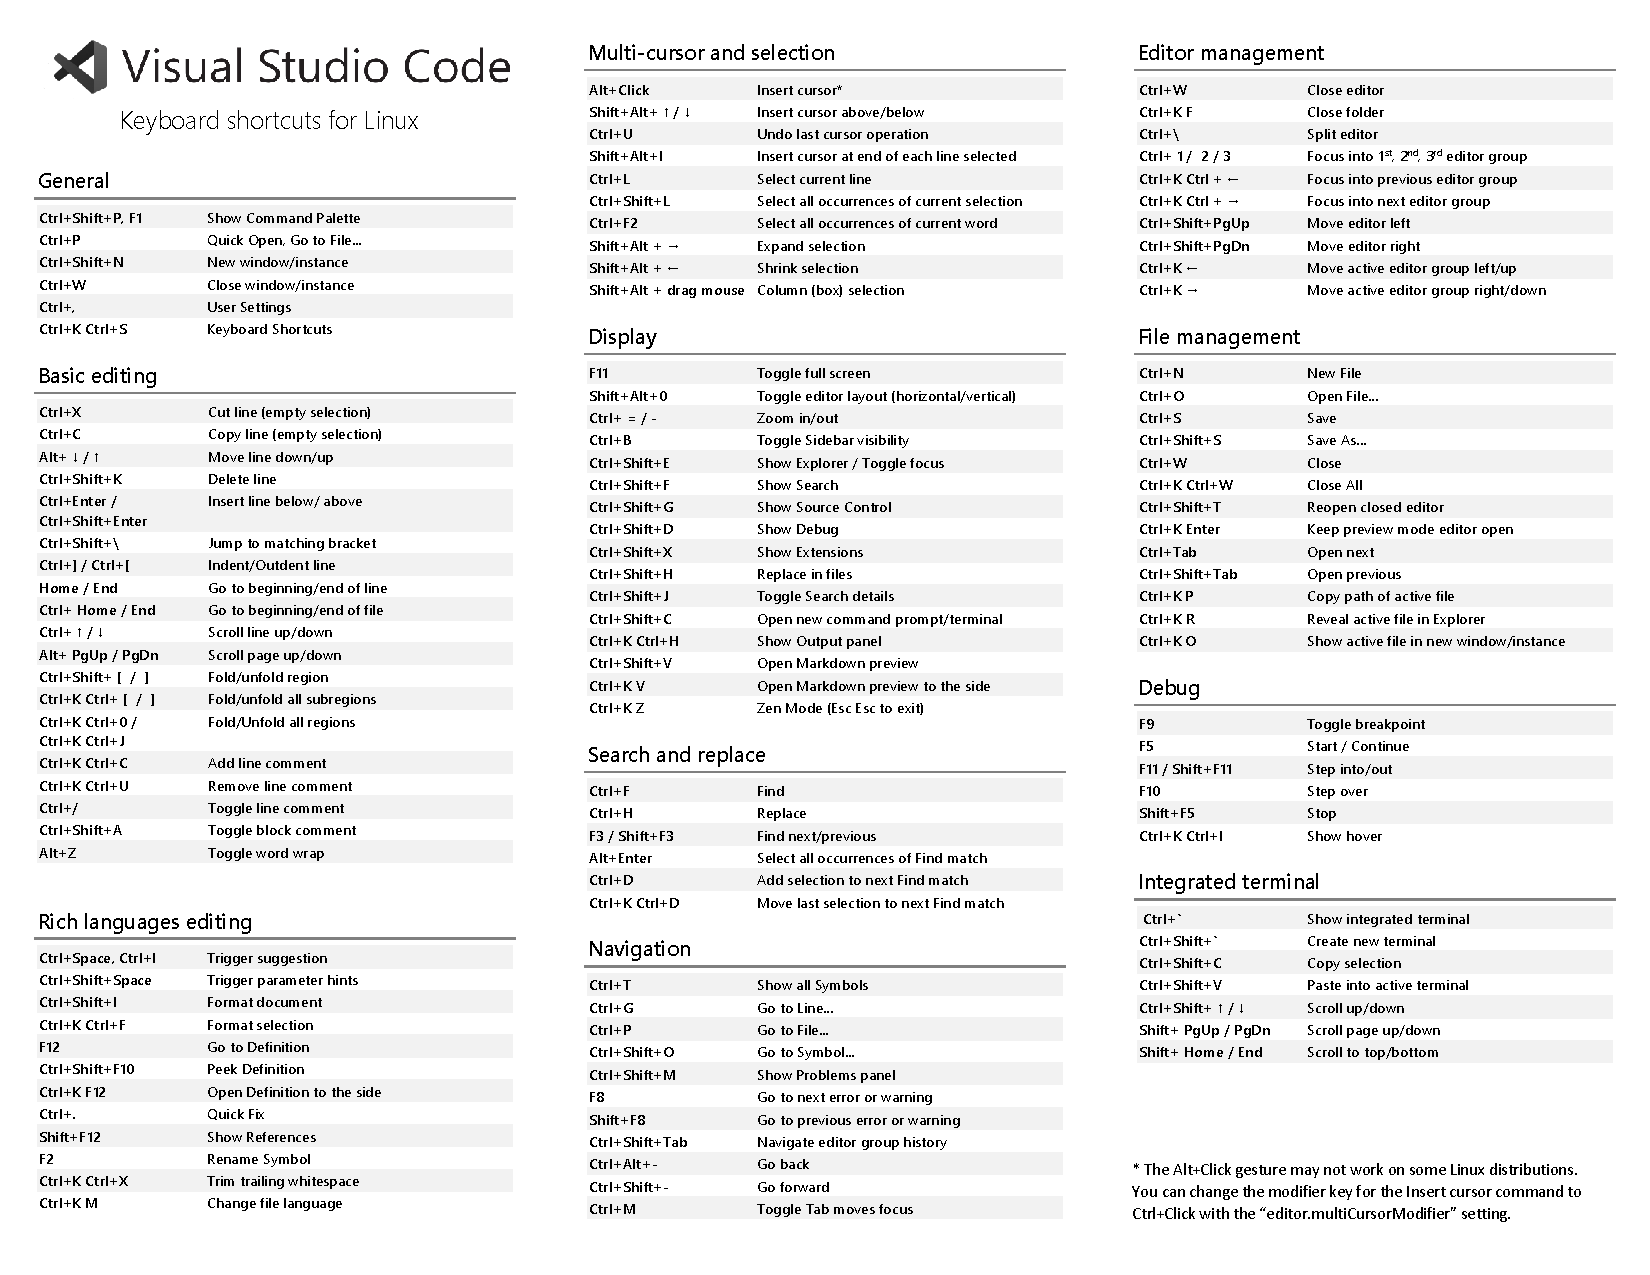
\includepdf[angle=270]{../src/misc/keyboard-shortcuts-linux.pdf}

	\pagestyle{empty}

	\newpage
	\ThisCenterWallPaper{1}{image/69150734_p0.jpg}

	\null

	\newpage
	\ThisCenterWallPaper{1}{image/72211605_p0.png}

	\null

	% \newpage
	% \ThisCenterWallPaper{1}{4.jpg}

	% \null
\end{document}
